\chapter{Diseño y construcción del robot}
\label{cap:capitulo5}

\begin{flushright}
\begin{minipage}[]{10cm}
\emph{La perfección se logra no cuando no hay nada más que añadir, sino cuando no hay nada más que quitar}\\
\end{minipage}\\

Antoine de Saint-Exupéry\\
\end{flushright}

\vspace{1cm}

Tras haber expuesto todas las plataformas de desarrollo utilizadas en este proyecto, en este capítulo se describirá el proceso paso a paso, desde la concepción inicial hasta la construcción y ensamblaje, para que el robot sea completamente operativo.

\section{Geometría del robot}
\label{sec:geometriarobot}

En este apartado se detalla el proceso llevado a cabo para definir la idea y la forma elegida para el robot. La aplicación de este proyecto se encuentra dentro de los robots de campo, y es por ello que estos tipos de robots son mayoritariamente plataformas que trabajan en entornos no estructurados, como se comentó en la Sección \ref{sec:robotcampo}. Por ello, es necesario que la estructura del robot se asemeje a esos tipos de robots y los más comunes son los robots con ruedas. 

Sin embargo, los robots de campo son de gran coste y de grandes dimensiones, lo que hacía inviable que entidades con recursos limitados pudieran adquirirlos. Es por ello que se decidió apostar por los robots de bajo coste. Una primera idea hasta conseguir la solución final al proyecto la tomamos del artículo, \cite{vega18c}, donde los autores nos presentan PiBot (Figura \ref{fig:pibot}), una plataforma robótica educativa de 20 x 10 x 8 cm basada en Raspberry Pi 3 y PiCamera, diseñada para facilitar la enseñanza de robótica a estudiantes de secundaria. Ofrece una infraestructura de \textit{software} abierta en Python y comandos de alto nivel para facilitar el aprendizaje. Además, incluye un modelo 3D imprimible y una versión simulada en Gazebo, disponibles públicamente para que estudiantes y escuelas puedan aprender y practicar robótica sin necesidad del robot físico. 

\begin{figure} [h!]
	\begin{center}
		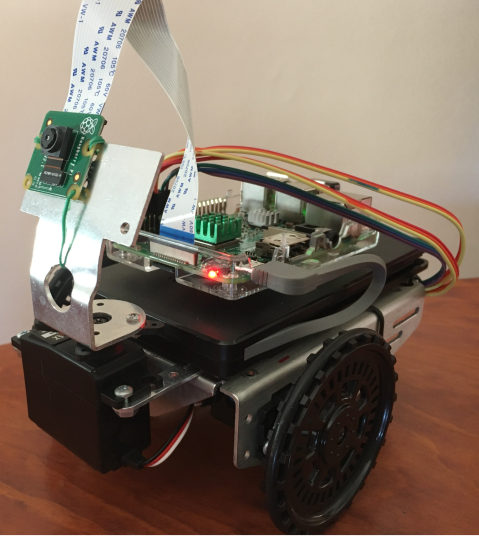
\includegraphics[width=6cm]{figs/cap5/Original.png}
	\end{center}
	\caption{PiBot} 
	\label{fig:pibot}
\end{figure}

Para poder continuar con la investigación de ese proyecto, se adquirió una unidad del robot PiBot. Además, se creó una estructura de metal para que la cámara cambiase su disposición, mirase hacia el suelo y estuviese orientada de forma natural para evitar futuros cálculos innecesarios. El diseño en este punto quedó como muestra la Figura \ref{fig:pibotmetal}.


\begin{figure} [h!]
	\begin{center}
		\includegraphics[width=8cm]{figs/cap5/new.png}
	\end{center}
	\caption{PiBot con cámara modificada} 
	\label{fig:pibotmetal}
\end{figure}


De PiBot interesa que tiene dos grados de libertad para el movimiento del robot, ya que cuenta con dos ruedas con motores independientes y una rueda loca, lo que le permite desplazarse a lo largo del eje X e Y y, por lo tanto, puede ir hacia delante y atrás y girar sobre sí mismo. Otro grado de libertad que resulta útil en PiBot para su aplicación en este proyecto es el giro sobre el eje Z del motor sobre el que está montada la cámara, lo que le permite aumentar el campo de visión (Figura \ref{fig:esquemaDOF}).


\begin{figure} [h!]
	\begin{center}
		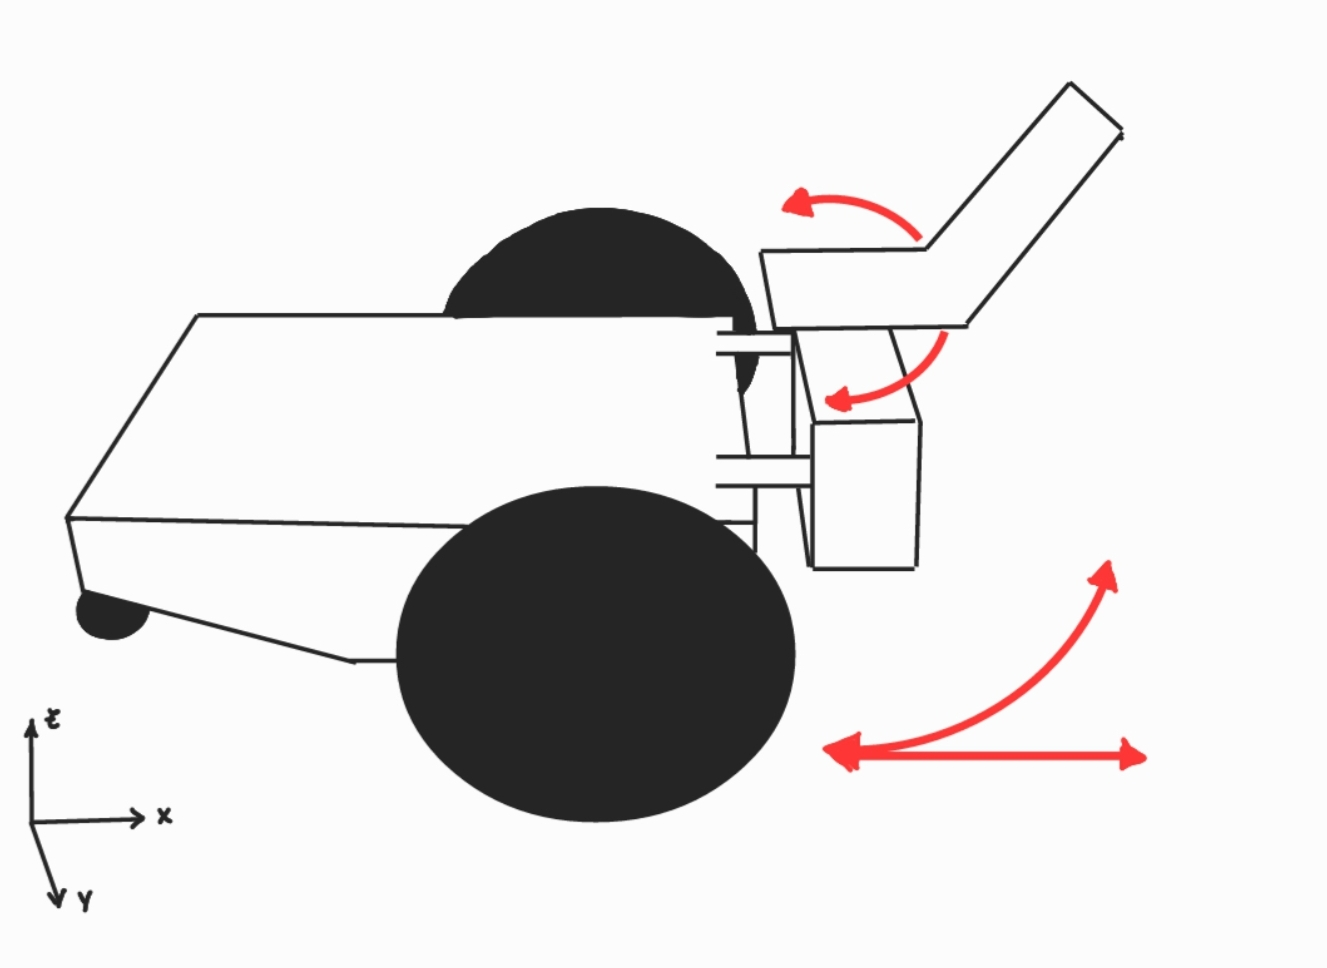
\includegraphics[width=9cm]{figs/cap5/dof.jpg}
	\end{center}
	\caption{Esquema de los grados de libertad de PiBot} 
	\label{fig:esquemaDOF}
\end{figure}


Una vez puesto en marcha el PiBot, se realizaron una serie de modificaciones \textit{hardware} para poder cumplir con el objetivo principal descrito en la Sección \ref{sec:descripcion}; fue necesario añadir una serie de componentes \textit{hardware} a PiBot para poder formar el esqueleto completo del nuevo prototipo robótico, que fue bautizado como PiBotJ. A continuación se describen detalladamente los distintos componentes \textit{hardware}.

\section{Disposición de los componentes hardware}
\label{sec:disposicionhardware}

Una vez conocido las características que eran útiles de PiBot para PiBotJ, se definió la disposición de los componentes \textit{hardware}, descritos en la Sección \ref{sec:hardware}, para poder confeccionar el esqueleto completo. La Figura \ref{fig:fritzzing} muestra todas la conexiones que fueron necesarias usar en la Raspberry Pi para dar soporte a todos los componentes del PiBotJ. 

\begin{figure} [h!]
	\begin{center}
		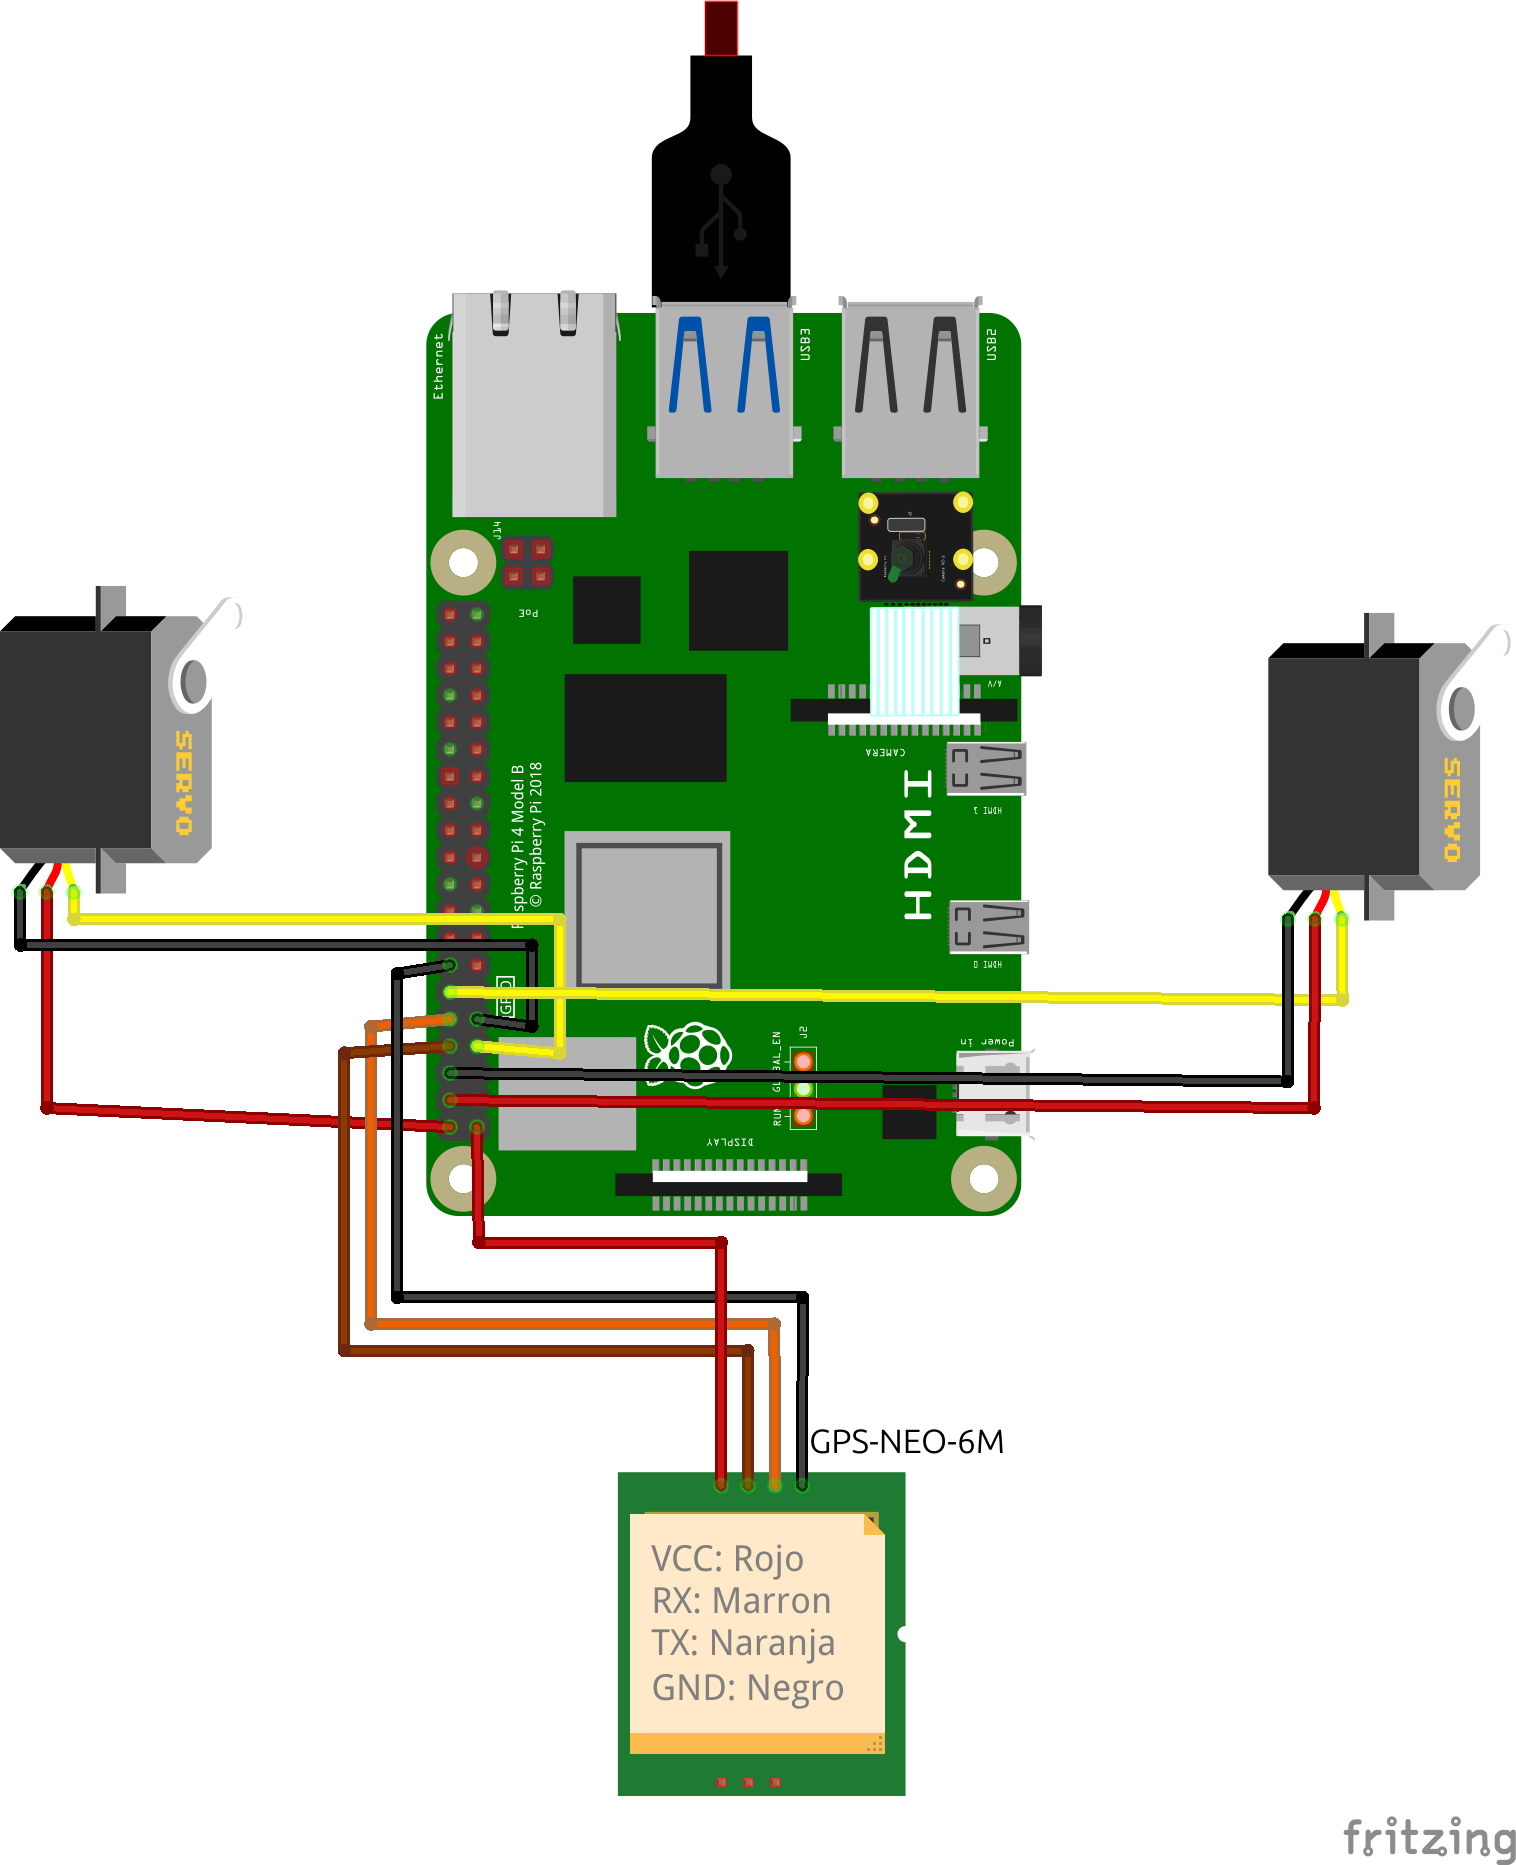
\includegraphics[width=10cm]{figs/cap5/modelocompleto_bb3.png}
	\end{center}
	\caption{Esquema de conexiones del PiBotJ} 
	\label{fig:fritzzing}
\end{figure}


La alimentación a la placa se realiza a través del puerto USB-C. En uno de los puertos USB 3.0 se conectó el Google Coral y, en el puerto CSI, la Raspberry PiCamera. Asimismo, sobre los pines se conectaron los servomotores estándar de Parallax y el módulo GPS. Para el servomotor derecho fue necesario usar el pin 4 para el cable de alimentación, el pin 12 (GPIO 18) para el cable de la señal y el pin 6 para el cable de tierra. Para el servomotor izquierdo fue necesario usar el pin 2 para el cable de alimentación, el pin 7 (GPIO 4) para el cable de la señal y el pin 9 para el cable de tierra. Finalmente, para el módulo GPS había que conectarlo al puerto serie y fue necesario usar el pin 1 para el cable de la alimentación, el pin 10 (GPIO 15) para el cable de transmisión de señal (TX), el pin 8 (GPIO 14) para el cable de recepción de señal (RX) y el pin 14 para el cable de tierra. 

 
\section{Bocetos}
\label{sec:bocetos}

La realización de bocetos es una etapa fundamental en el proceso de diseño, que se realiza antes de iniciar el modelado en 3D, ya que su propósito es obtener una visión clara de la estructura y disposición de los componentes que conforman el PiBotJ. Una vez que se definió el esqueleto completo que este necesitaba, se creó una serie de bocetos (Figura \ref{fig:bocetos}) que permitieron afinar los detalles antes de realizar el diseño en 3D.

\begin{figure}[ht!]
	\centering
	\begin{minipage}{0.4\linewidth}
		\centering
		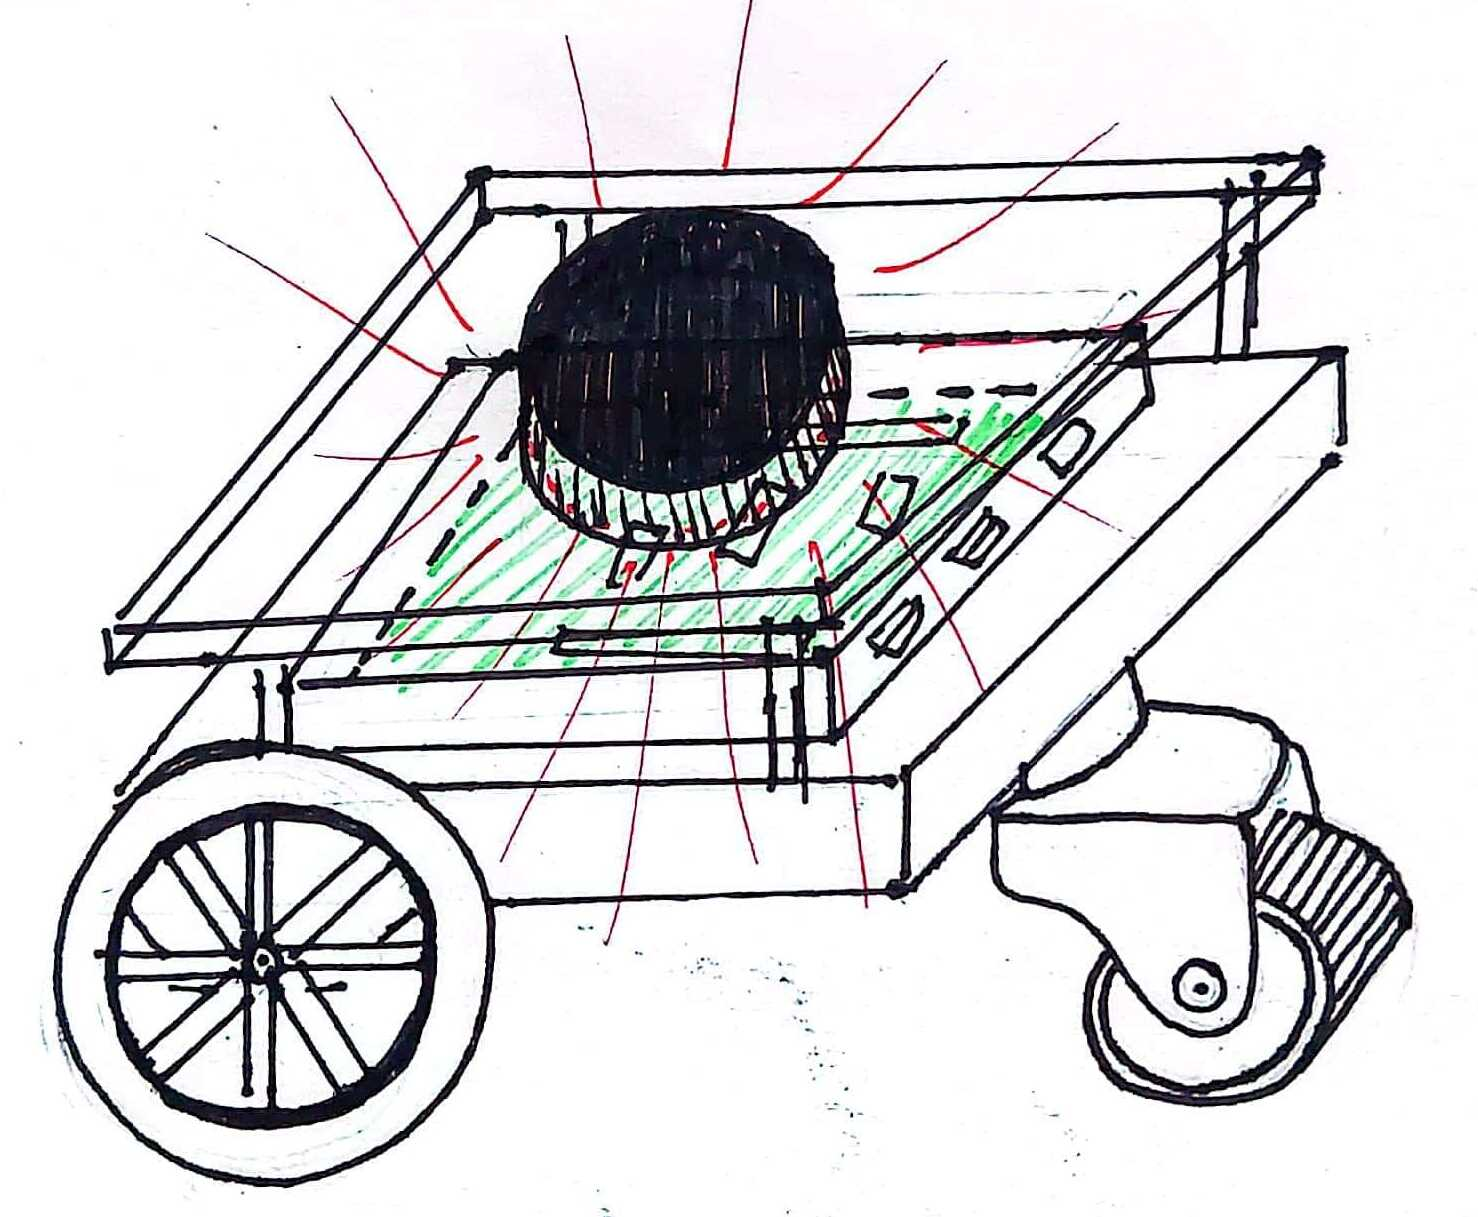
\includegraphics[width=\linewidth]{figs/cap5/prototipo_laser.jpeg}
	\end{minipage}
	\hspace{2cm}
	\begin{minipage}{0.4\linewidth}
		\centering
		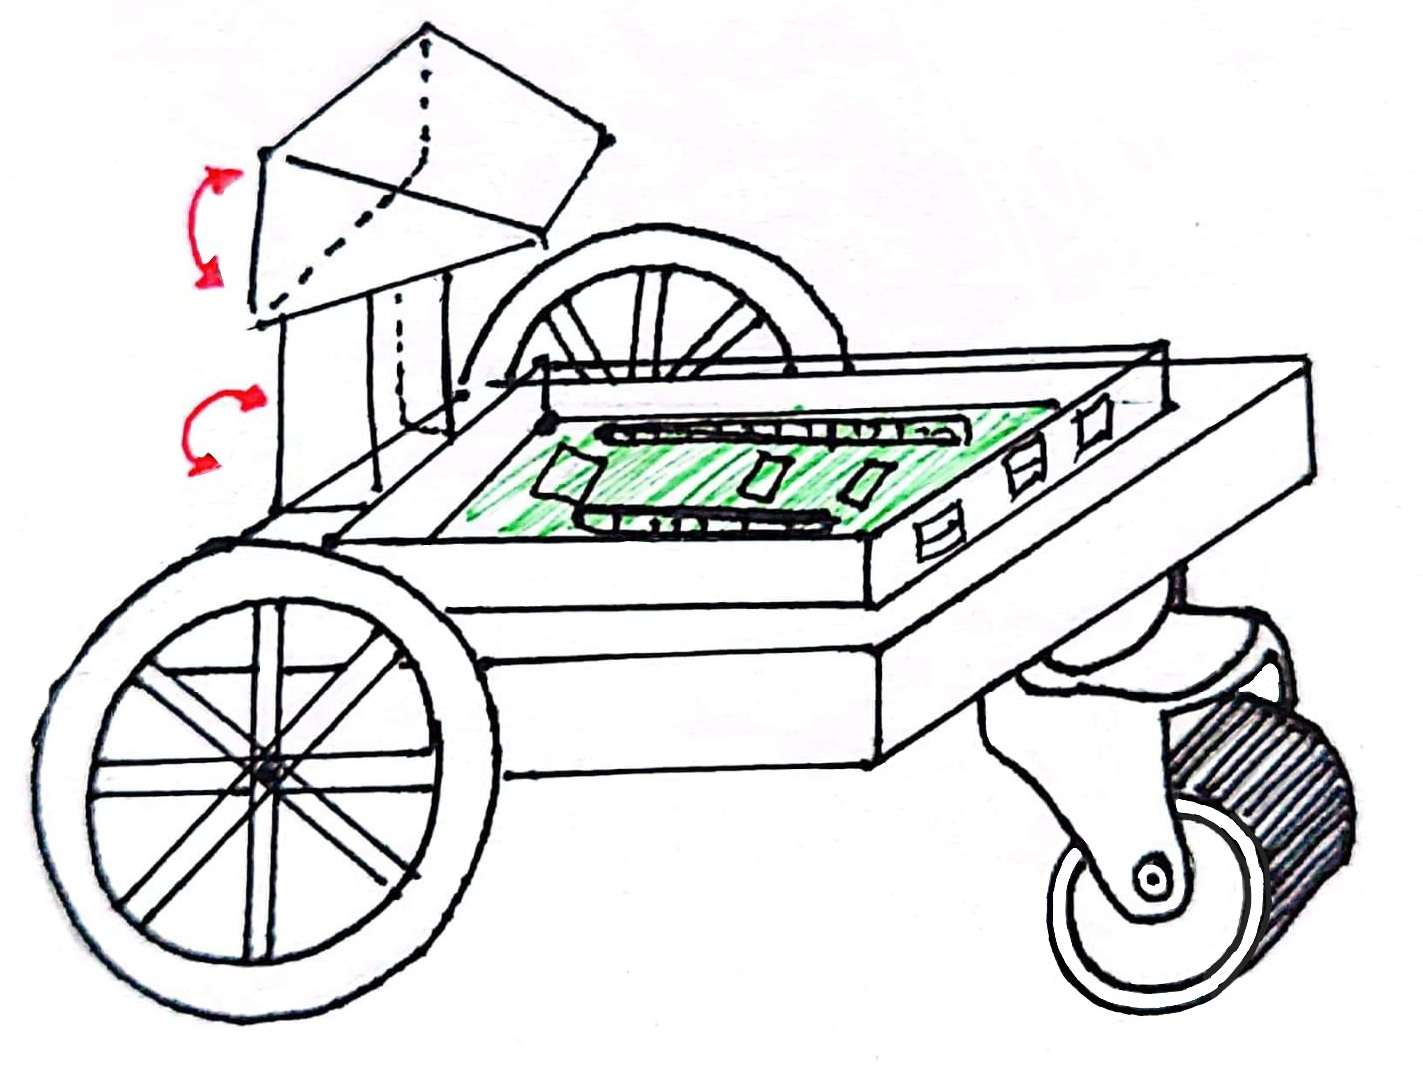
\includegraphics[width=\linewidth]{figs/cap5/prototipo_sin_laser.jpeg}
	\end{minipage}
	\hspace{2cm}
	\begin{minipage}{0.5\linewidth}
		\centering
		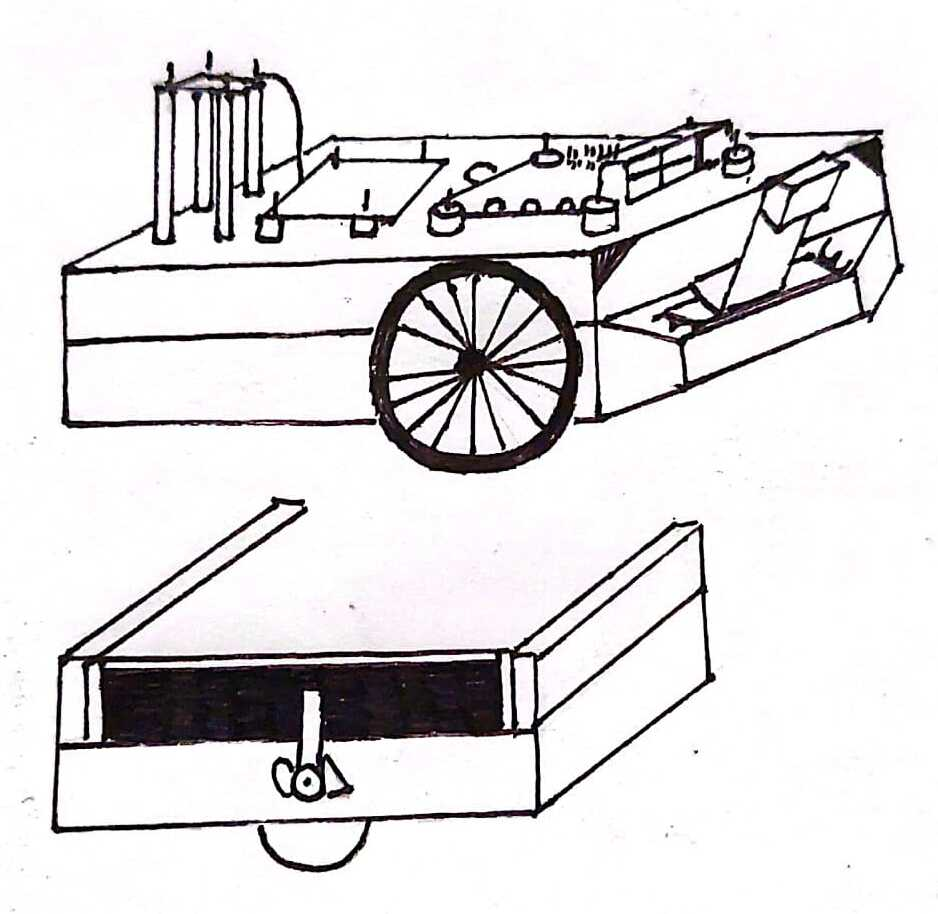
\includegraphics[width=\linewidth]{figs/cap5/boceto_papel.jpeg}
	\end{minipage}
	\caption{Bocetos creados a mano}
	\label{fig:bocetos}
\end{figure}

Antes de realizar el diseño \acs{CAD} de las piezas se creó una maqueta a tamaño real (Figura \ref{fig:maqueta2}) para poder tener una idea de cómo sería la aplicación final y así intentar no malgastar material de impresión. Tras tener una idea clara de cómo iba a ser PiBotJ, se comenzó con el diseño de cada una de las piezas.  

%\begin{figure}[ht!]
%	\centering
%	\begin{minipage}{0.5\linewidth}
%		\centering
%		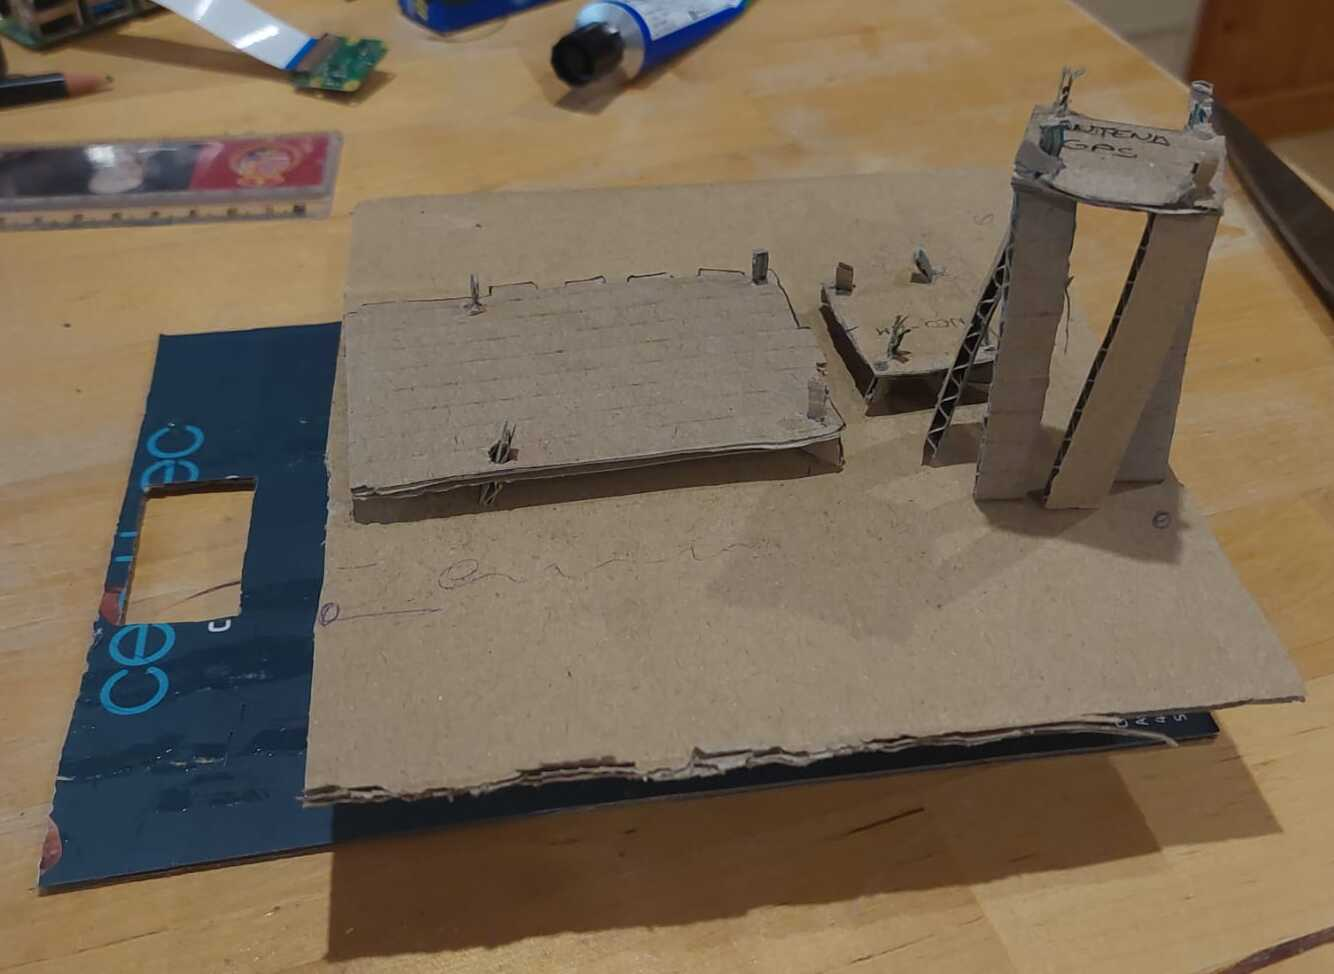
\includegraphics[width=\linewidth]{figs/cap5/boceto_carton1.jpeg}
%		\caption*{\centering}
%	\end{minipage}
%	\hspace{1cm}
%	\begin{minipage}{0.4\linewidth}
%		\centering
%		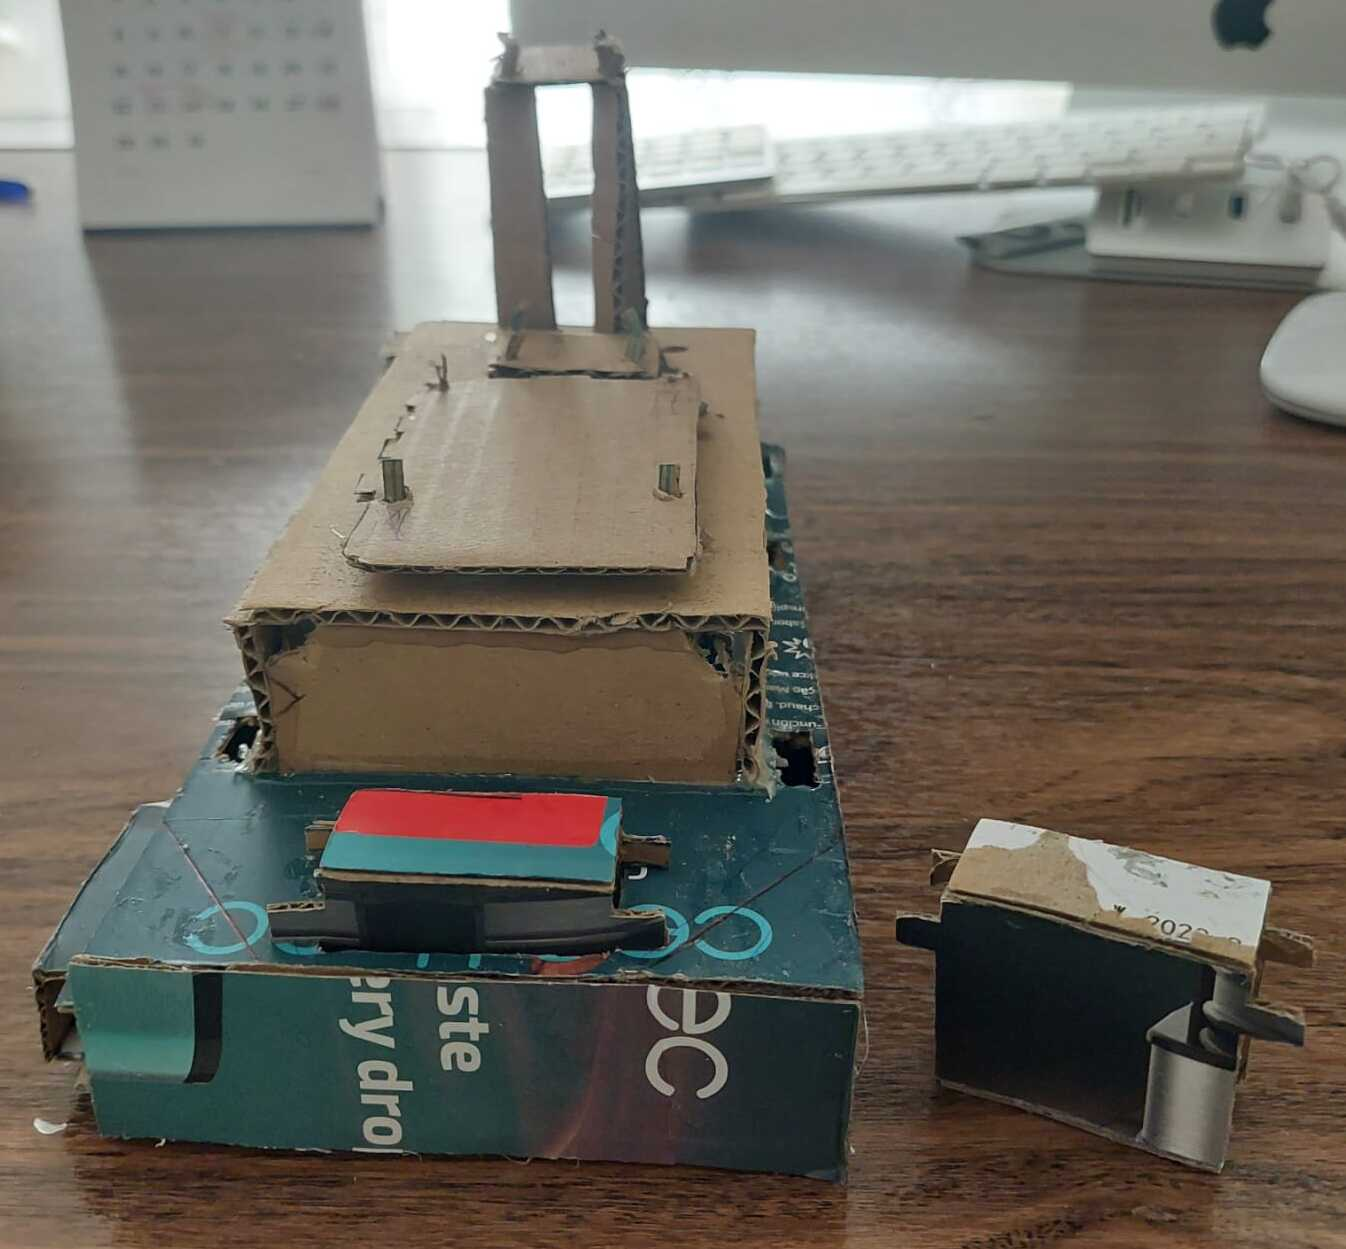
\includegraphics[width=\linewidth]{figs/cap5/boceto_carton2.jpeg}
%		\caption*{\centering}
%	\end{minipage}
%	\hspace{2cm}
%	\begin{minipage}{0.4\linewidth}
%		\centering
%		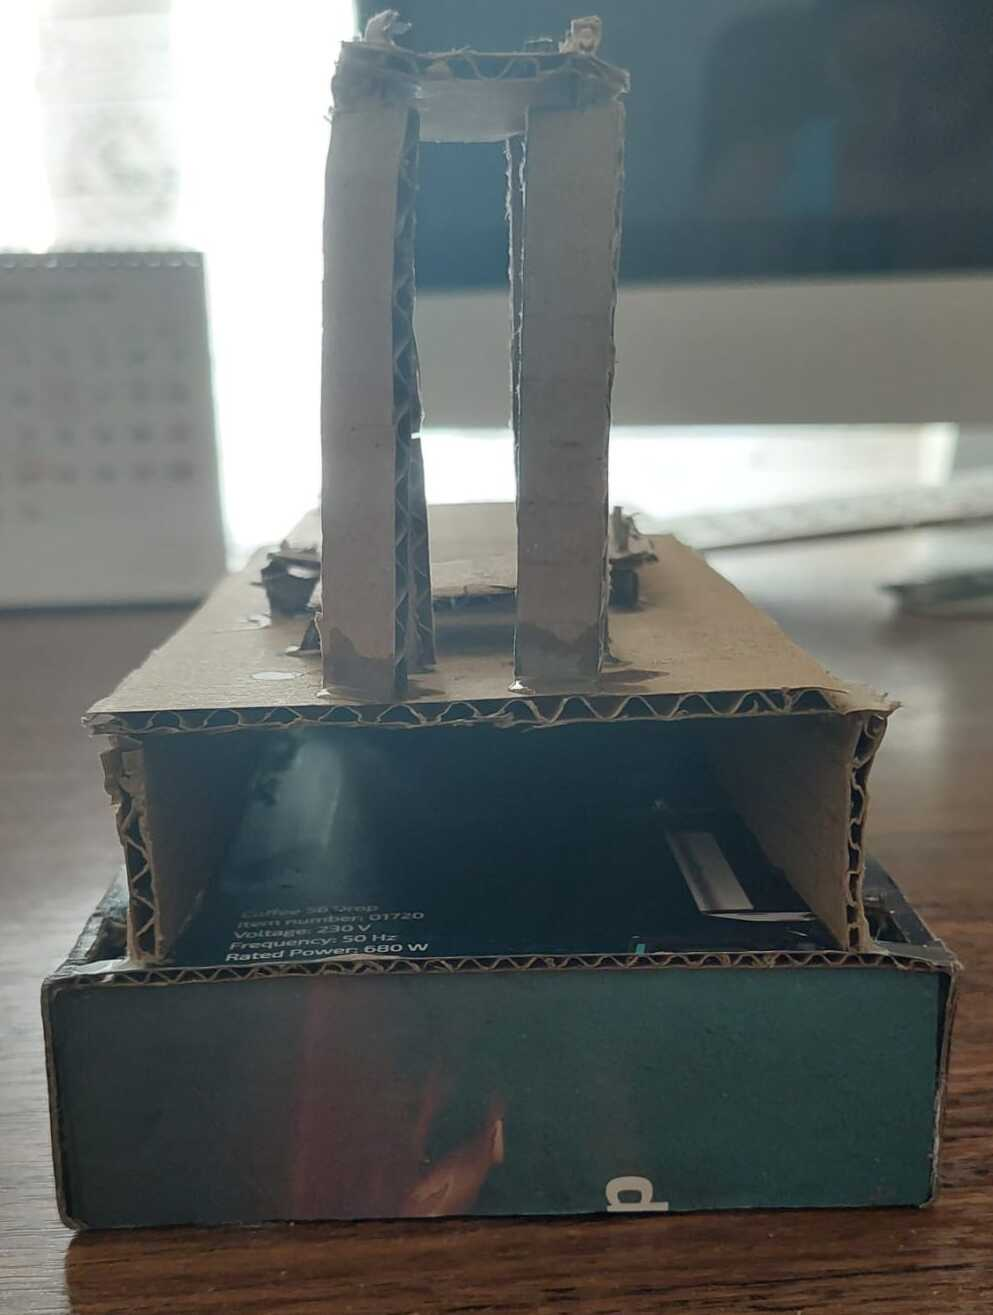
\includegraphics[width=\linewidth]{figs/cap5/boceto_carton3.jpeg}
%		\caption*{\centering}
%	\end{minipage}
%	\caption{Maqueta en proceso}
%	\label{fig:maqueta1}
%\end{figure}

\begin{figure}[ht!]
	\centering
	%\begin{minipage}{0.44\linewidth}
	%	\centering
	%	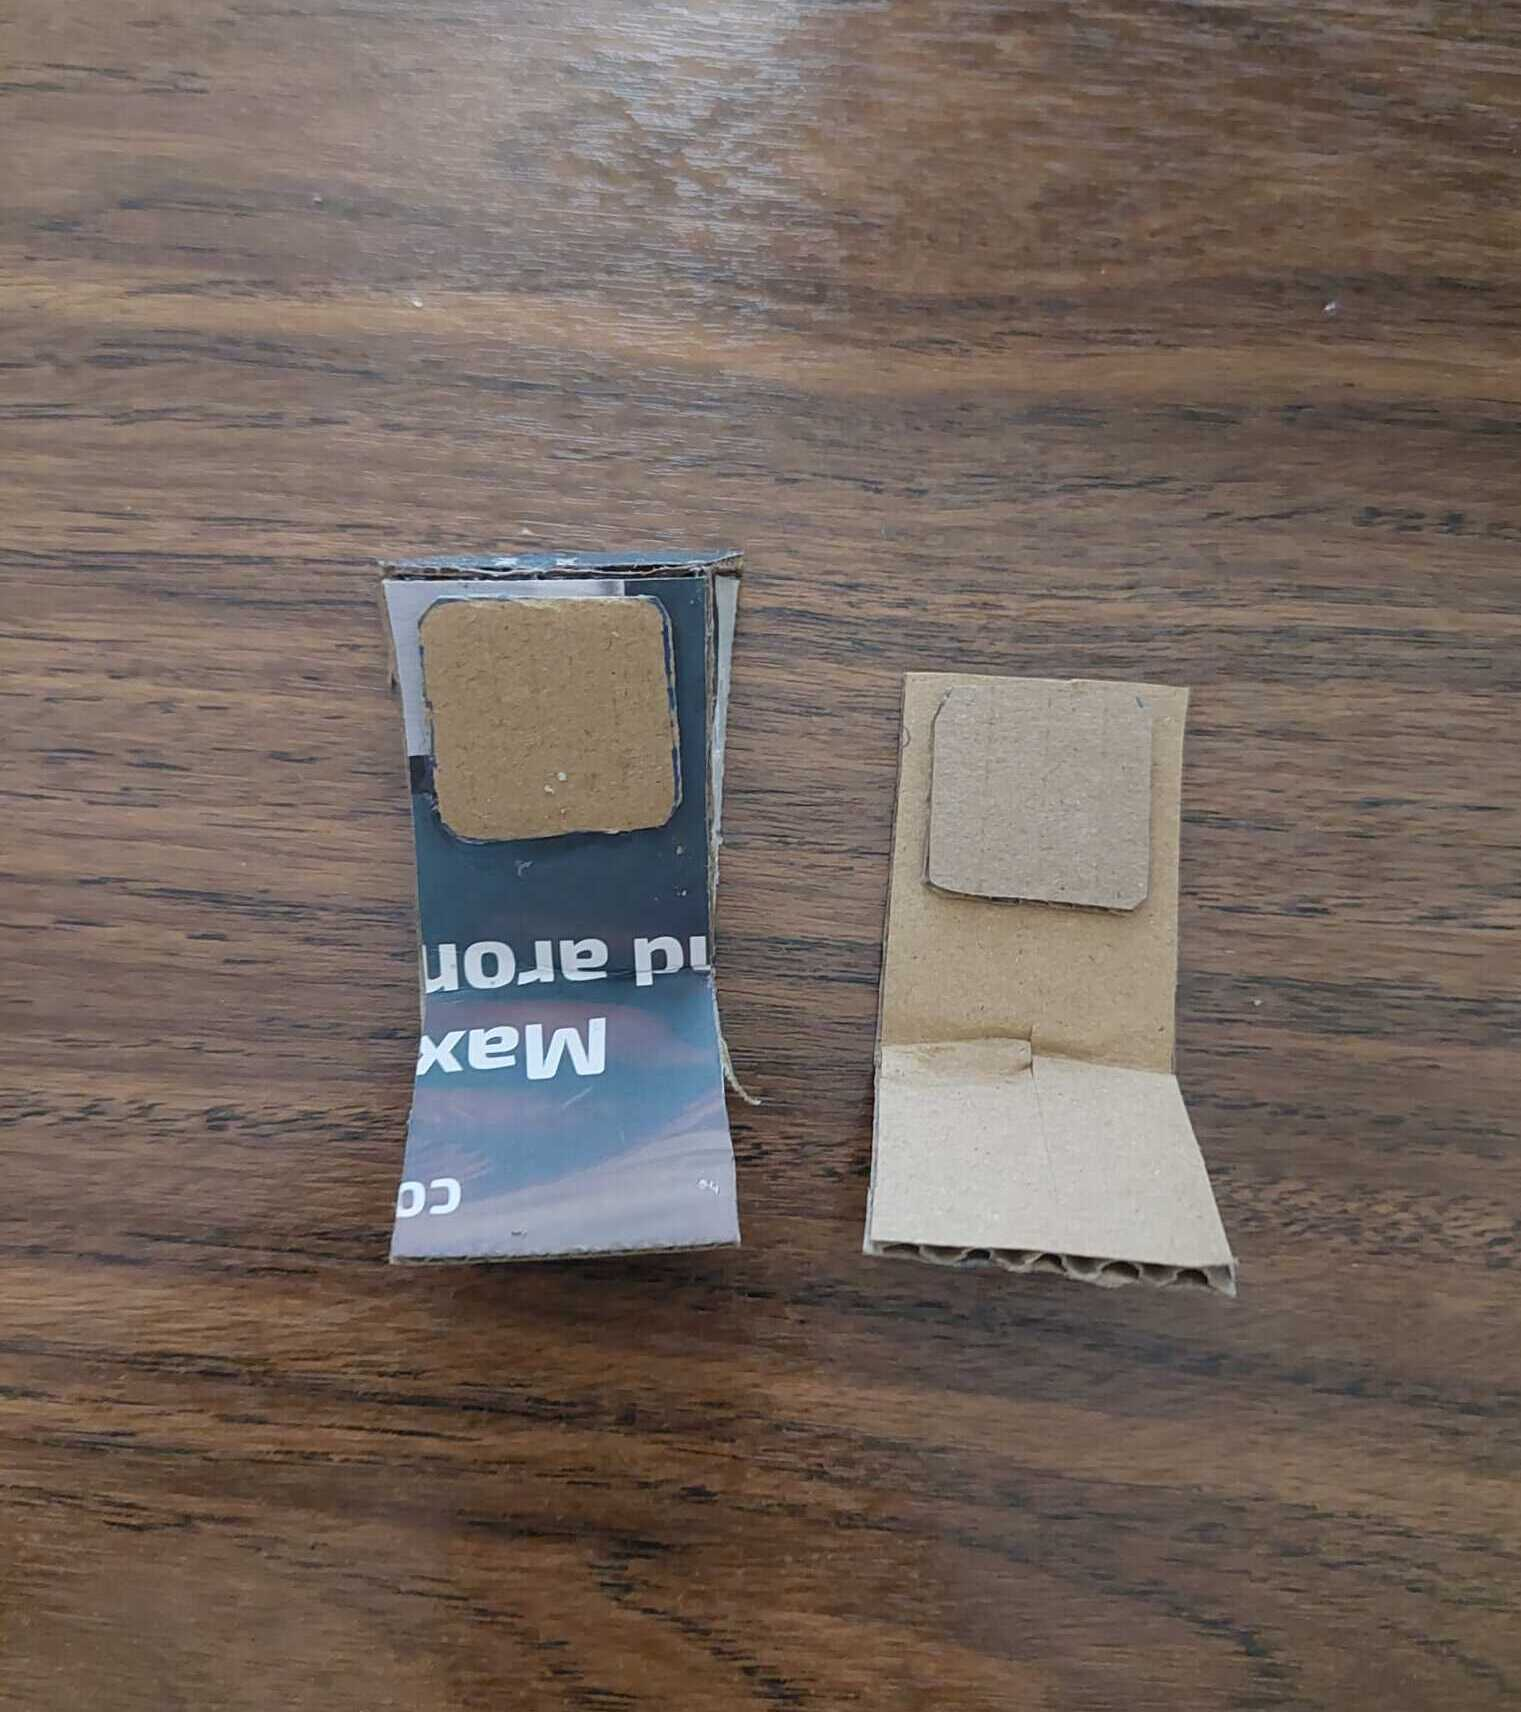
\includegraphics[width=\linewidth]{figs/cap5/boceto_carton4.jpeg}
	%	\caption*{\centering}
	%\end{minipage}
	%\hspace{2cm}
	\begin{minipage}{0.4\linewidth}
		\centering
		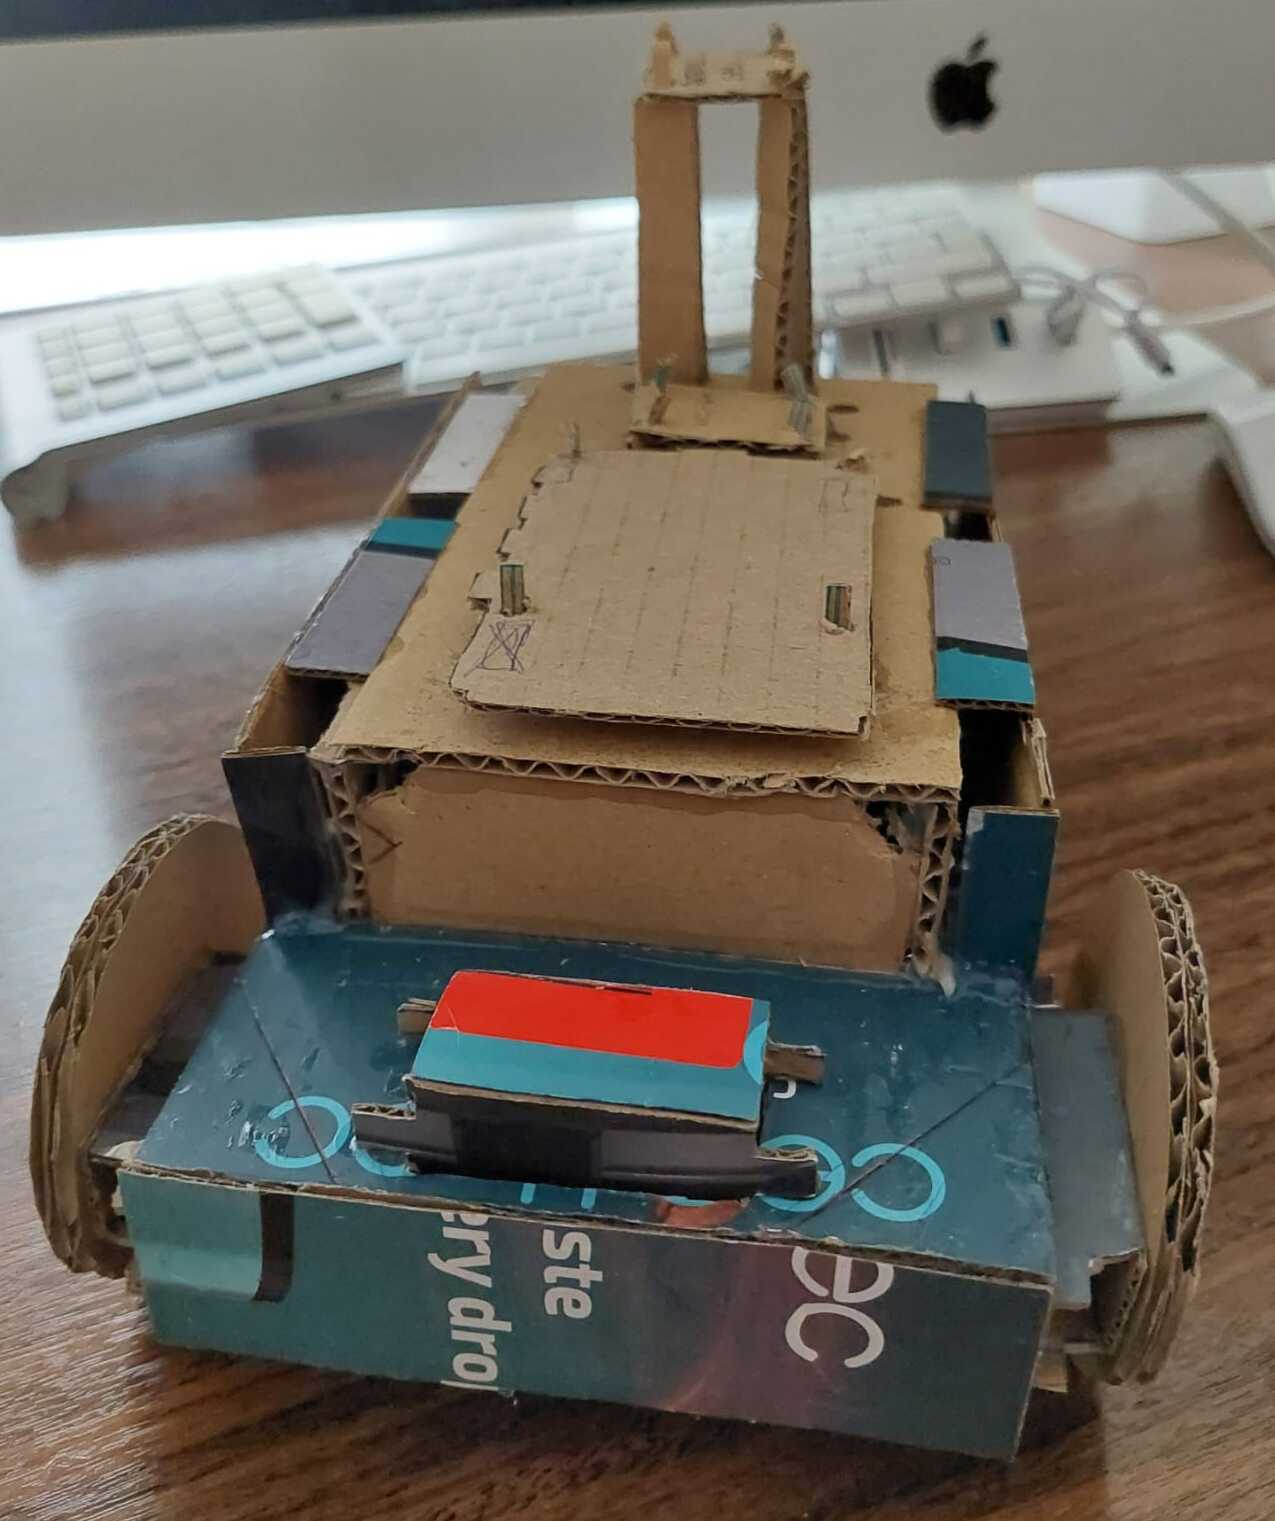
\includegraphics[width=\linewidth]{figs/cap5/boceto_carton5.jpeg}
		%\caption*{\centering}
	\end{minipage}
	\hspace{2cm}
	%\begin{minipage}{0.45\linewidth}
	%	\centering
	%	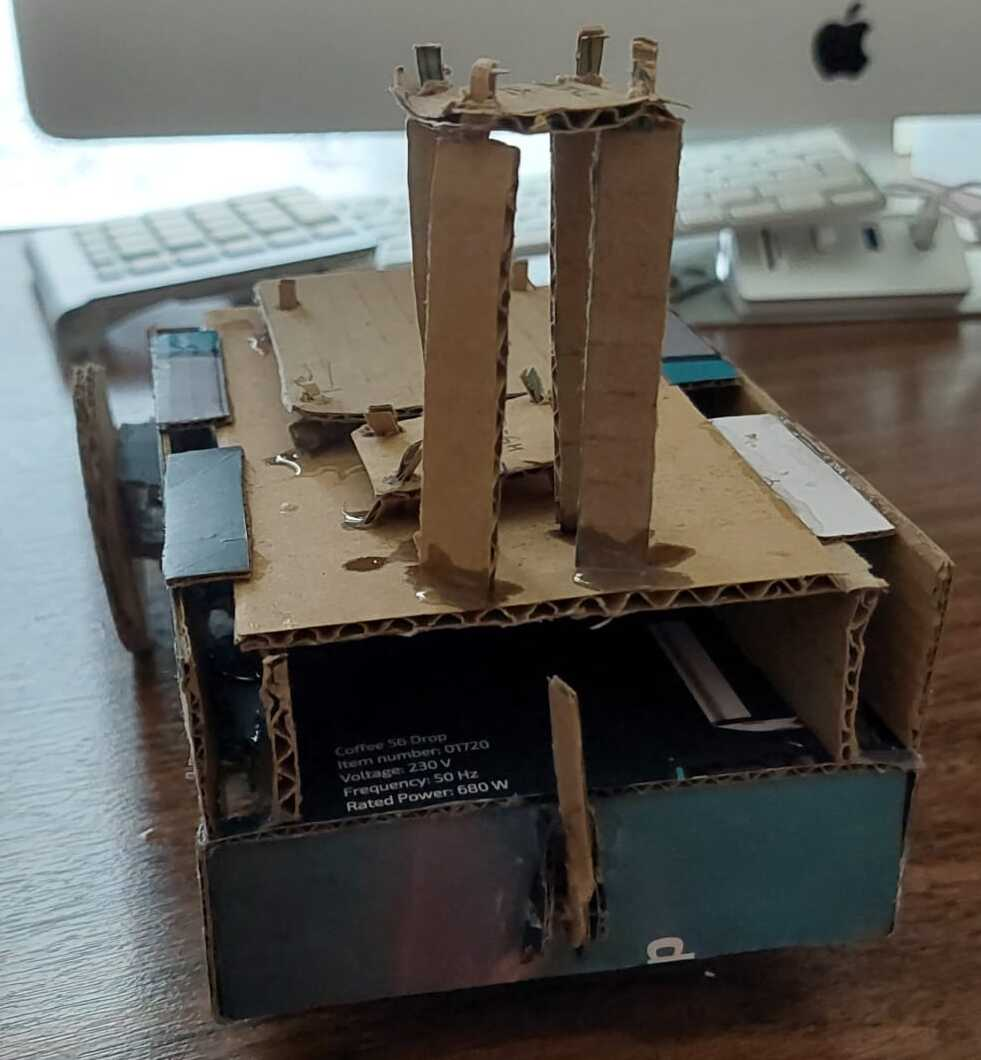
\includegraphics[width=\linewidth]{figs/cap5/boceto_carton6.jpeg}
	%	\caption*{\centering}
	%\end{minipage}
	%\hspace{2cm}
	\begin{minipage}{0.4\linewidth}
		\centering
		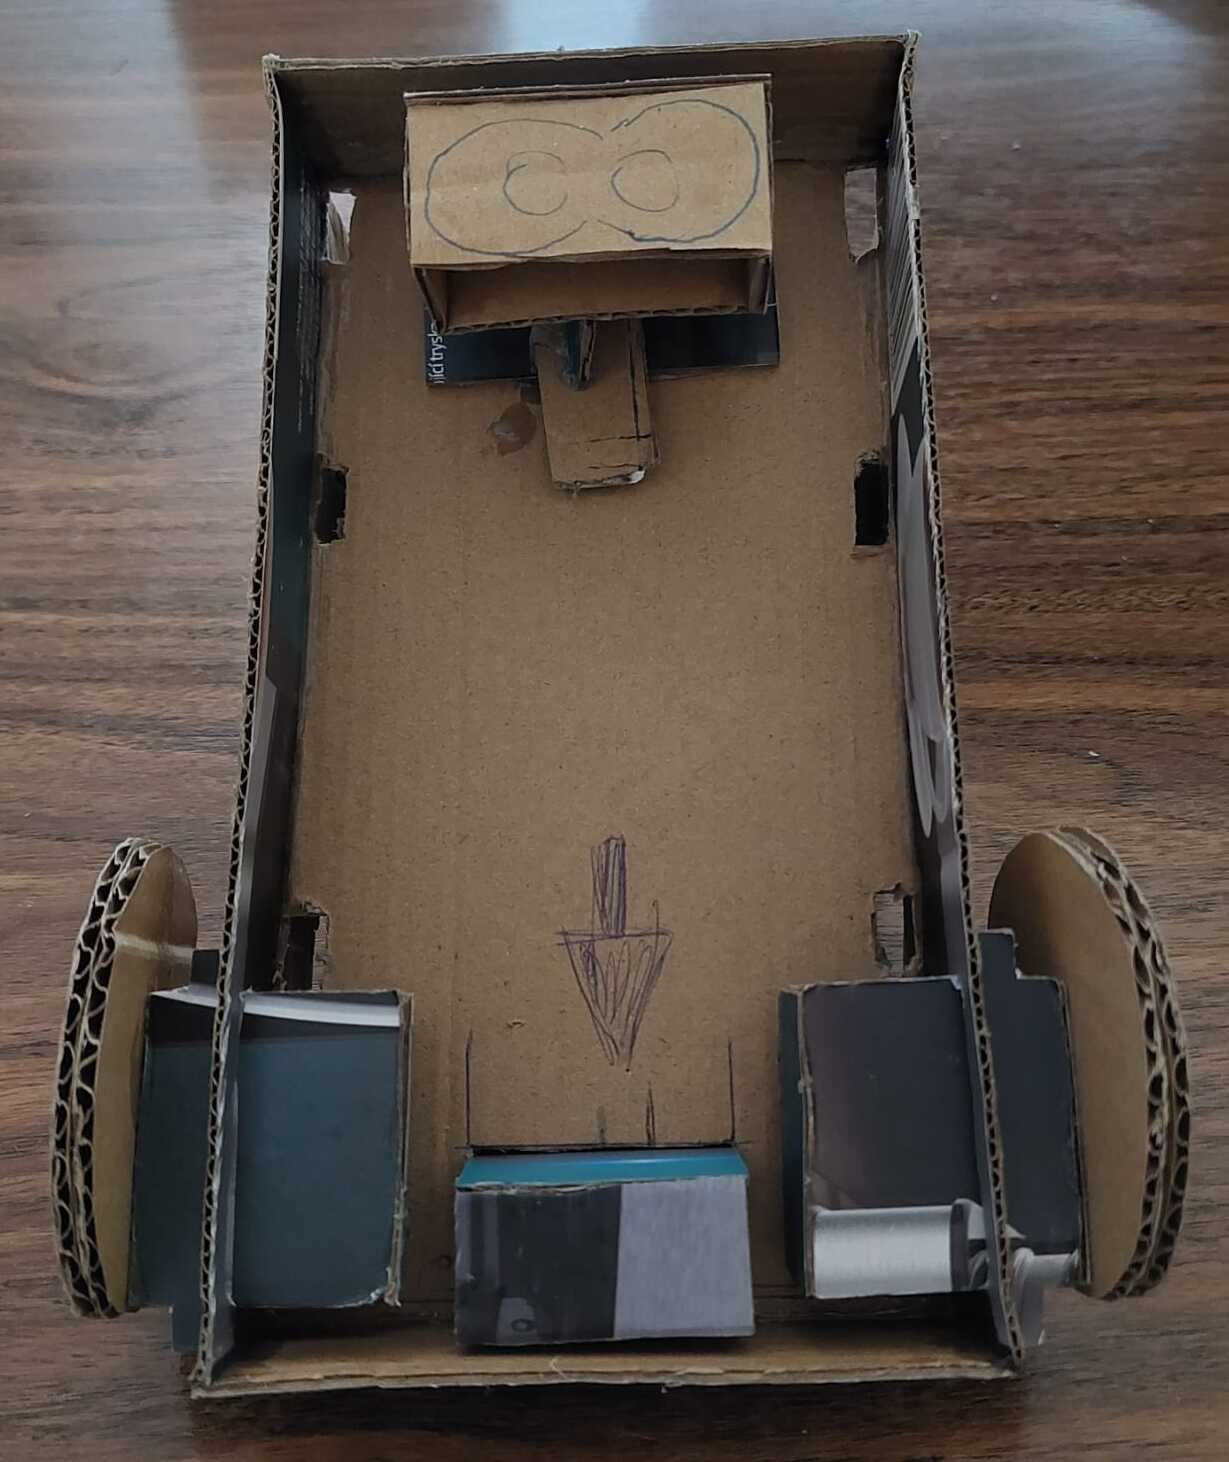
\includegraphics[width=\linewidth]{figs/cap5/boceto_carton7.jpeg}
		%\caption*{\centering}
	\end{minipage}
	\caption{Maqueta creada}
	\label{fig:maqueta2}
\end{figure}


\section{Diseño CAD}
\label{sec:diseñocad}

Para hacer el diseño \acs{CAD} y la maqueta explicada en el apartado anterior, se crearon unos planos a mano (Figura \ref{fig:planos}) de las diferentes piezas involucradas en el diseño. Las medidas fueron precisas gracias al uso del calibre.


\begin{figure}[ht!]
	\centering
	\begin{minipage}{0.45\linewidth}
		\centering
		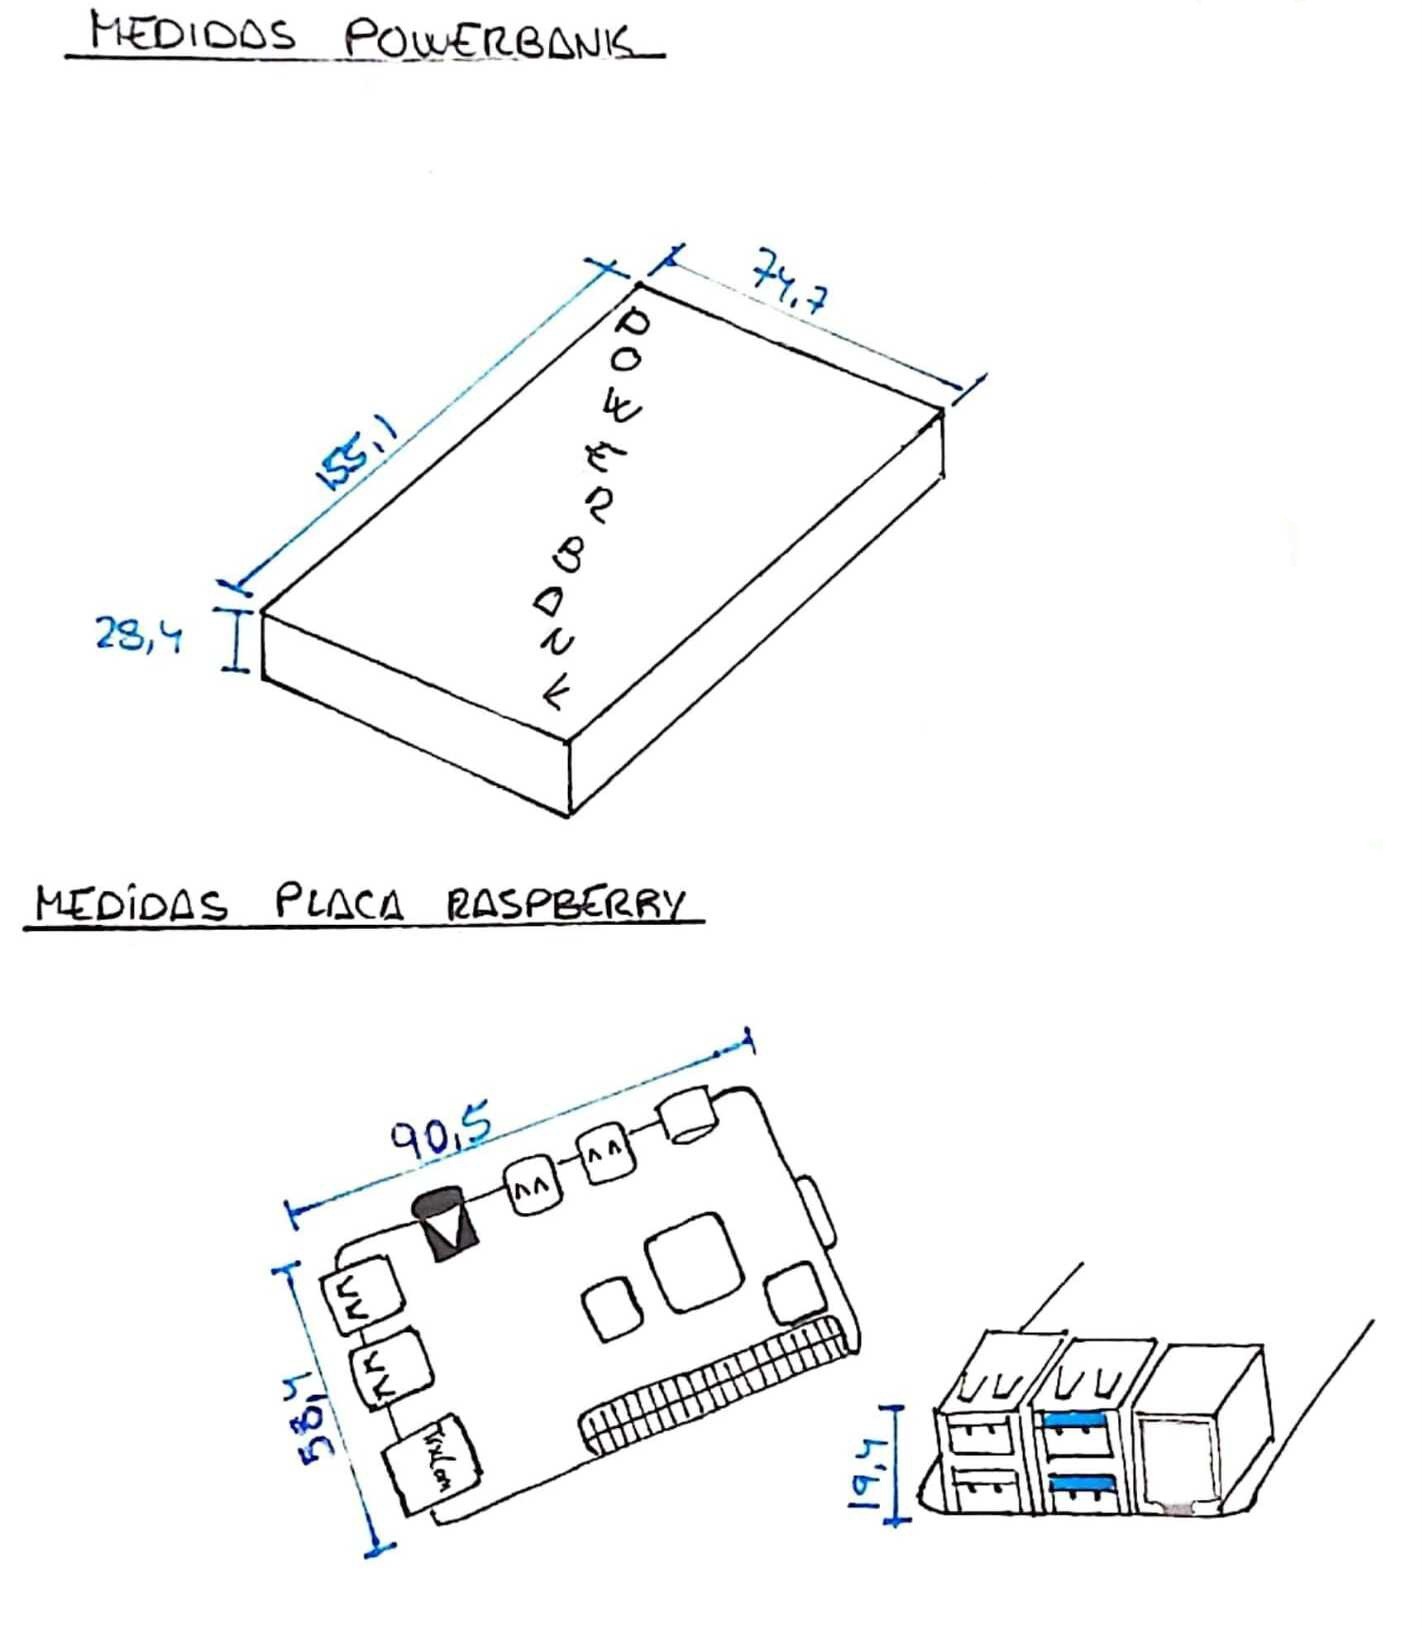
\includegraphics[width=\linewidth]{figs/cap5/planos1.jpeg}
		\caption*{\centering}
	\end{minipage}
	\hspace{1cm}
	\begin{minipage}{0.45\linewidth}
		\centering
		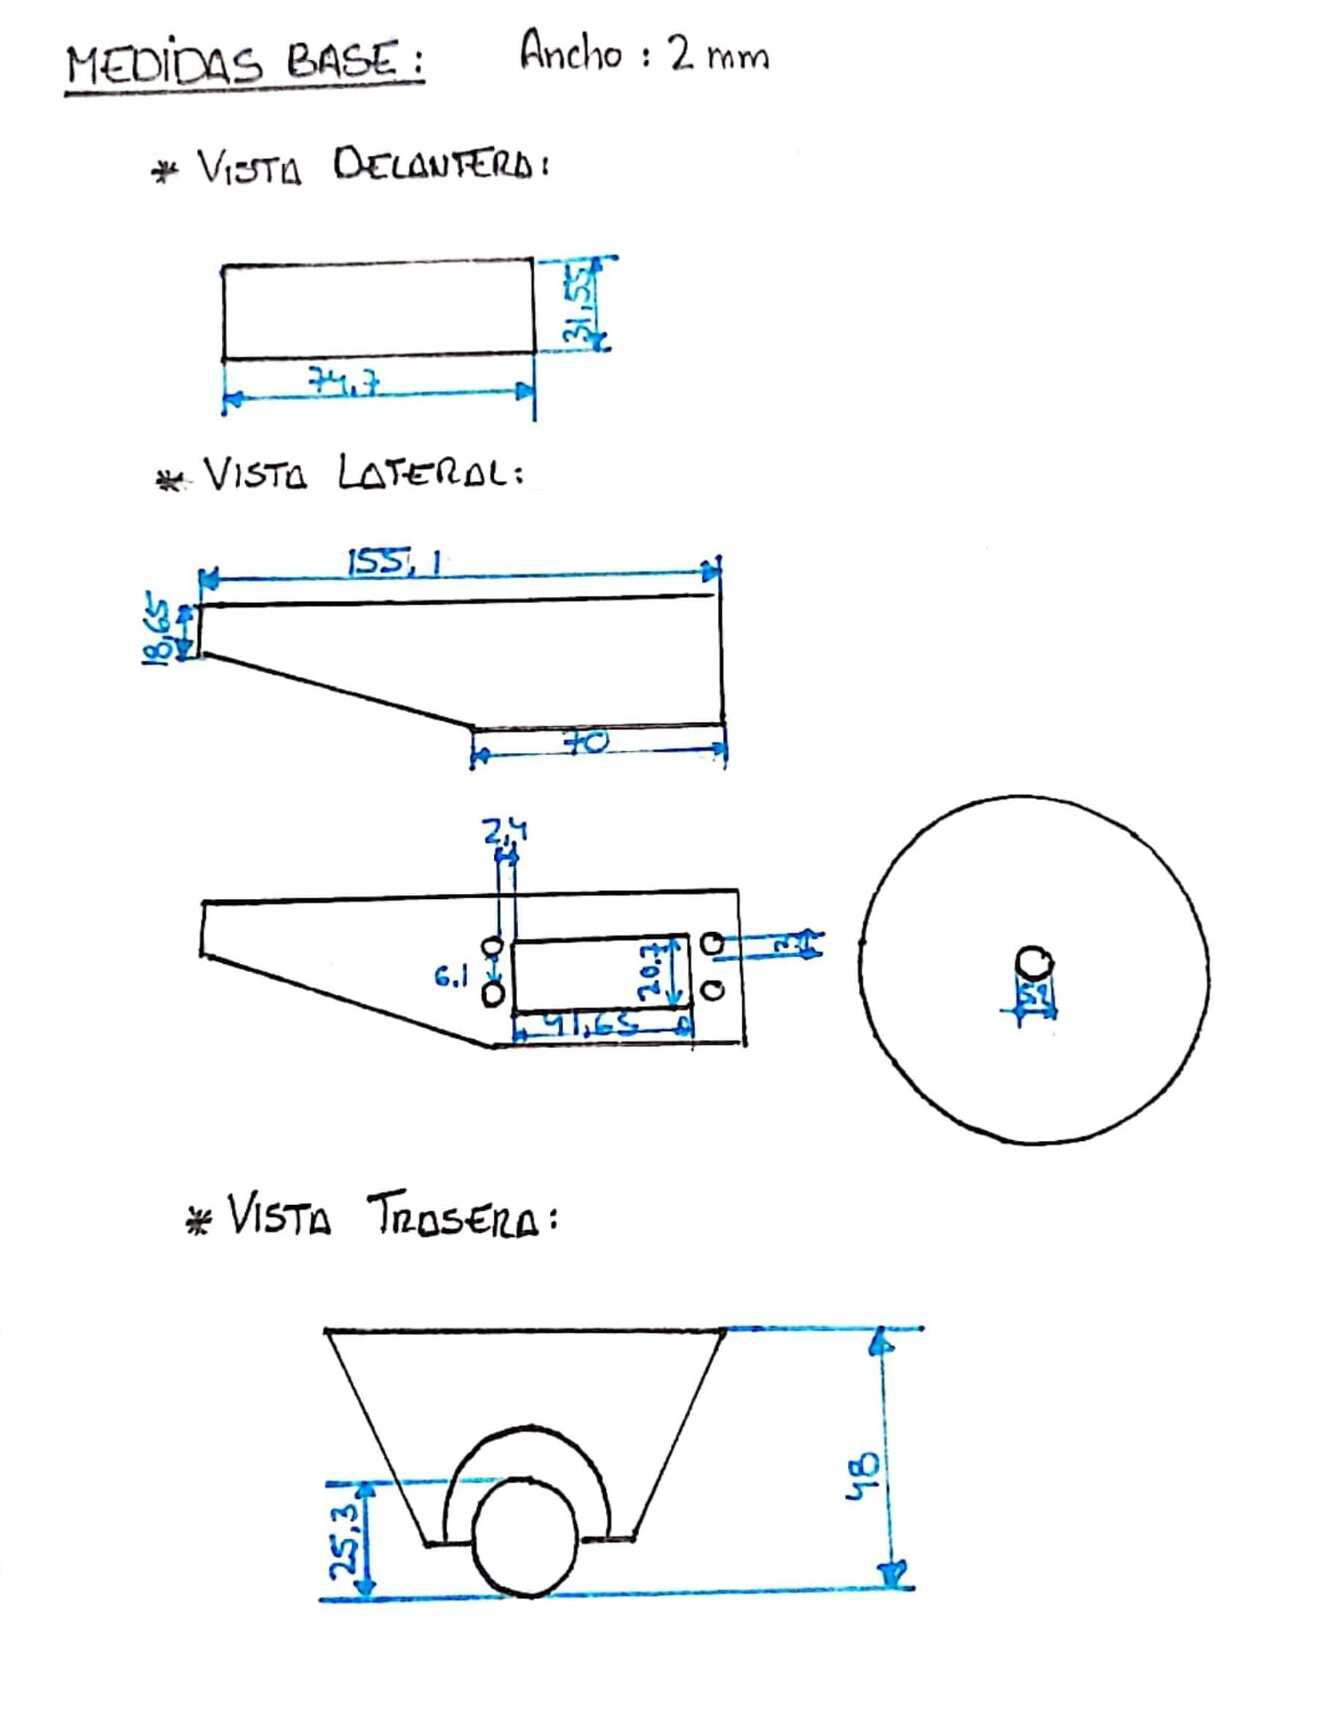
\includegraphics[width=\linewidth]{figs/cap5/planos2.jpeg}
		\caption*{\centering}
	\end{minipage}
	\hspace{1cm}
	\begin{minipage}{0.45\linewidth}
		\centering
		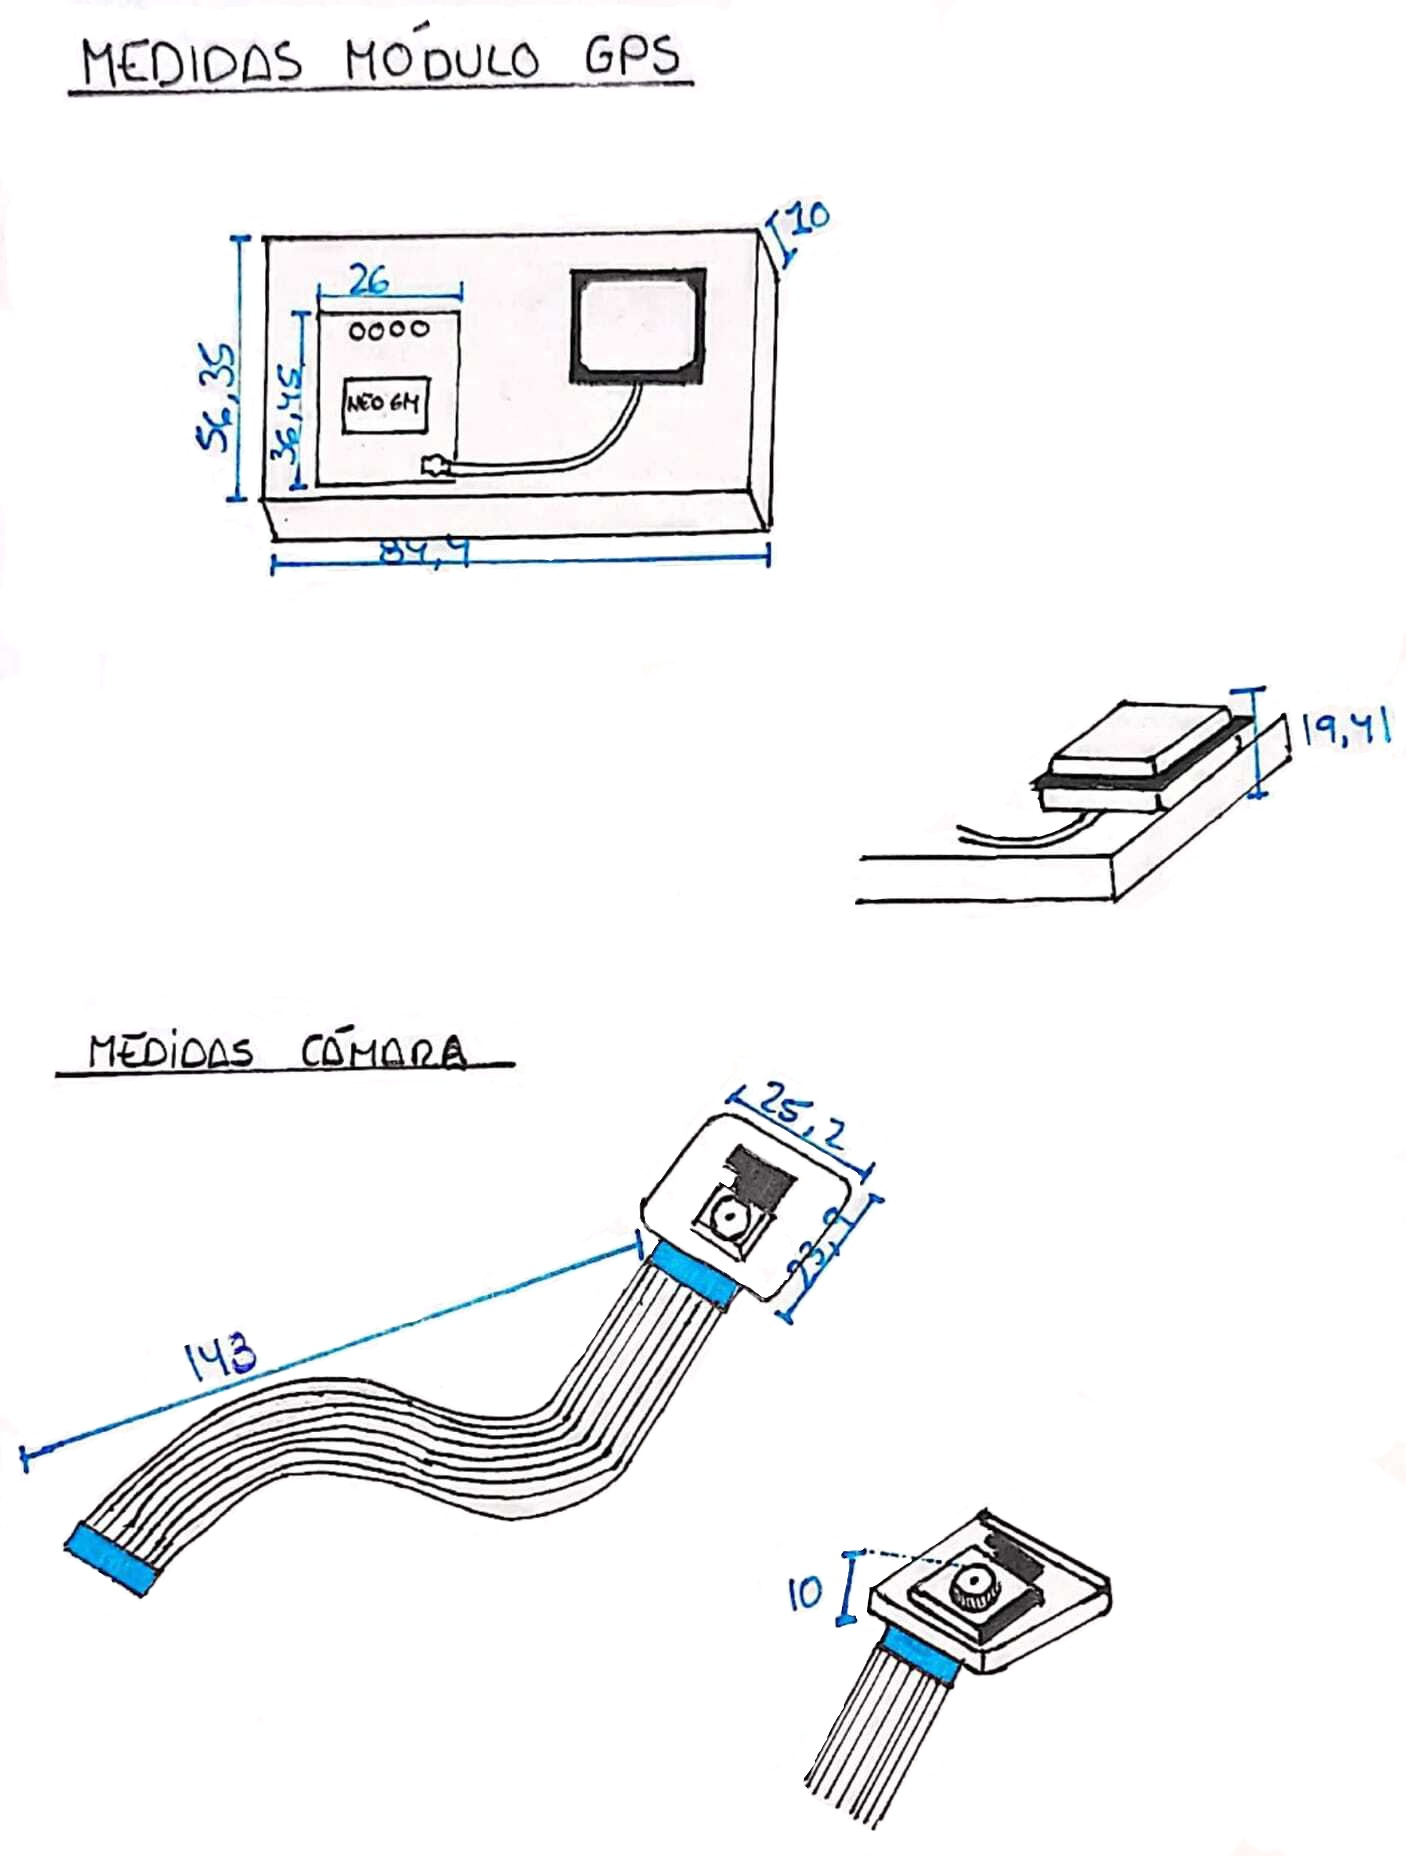
\includegraphics[width=\linewidth]{figs/cap5/planos3.jpeg}
		\caption*{\centering}
	\end{minipage}
	\hspace{1cm}
	\begin{minipage}{0.45\linewidth}
		\centering
		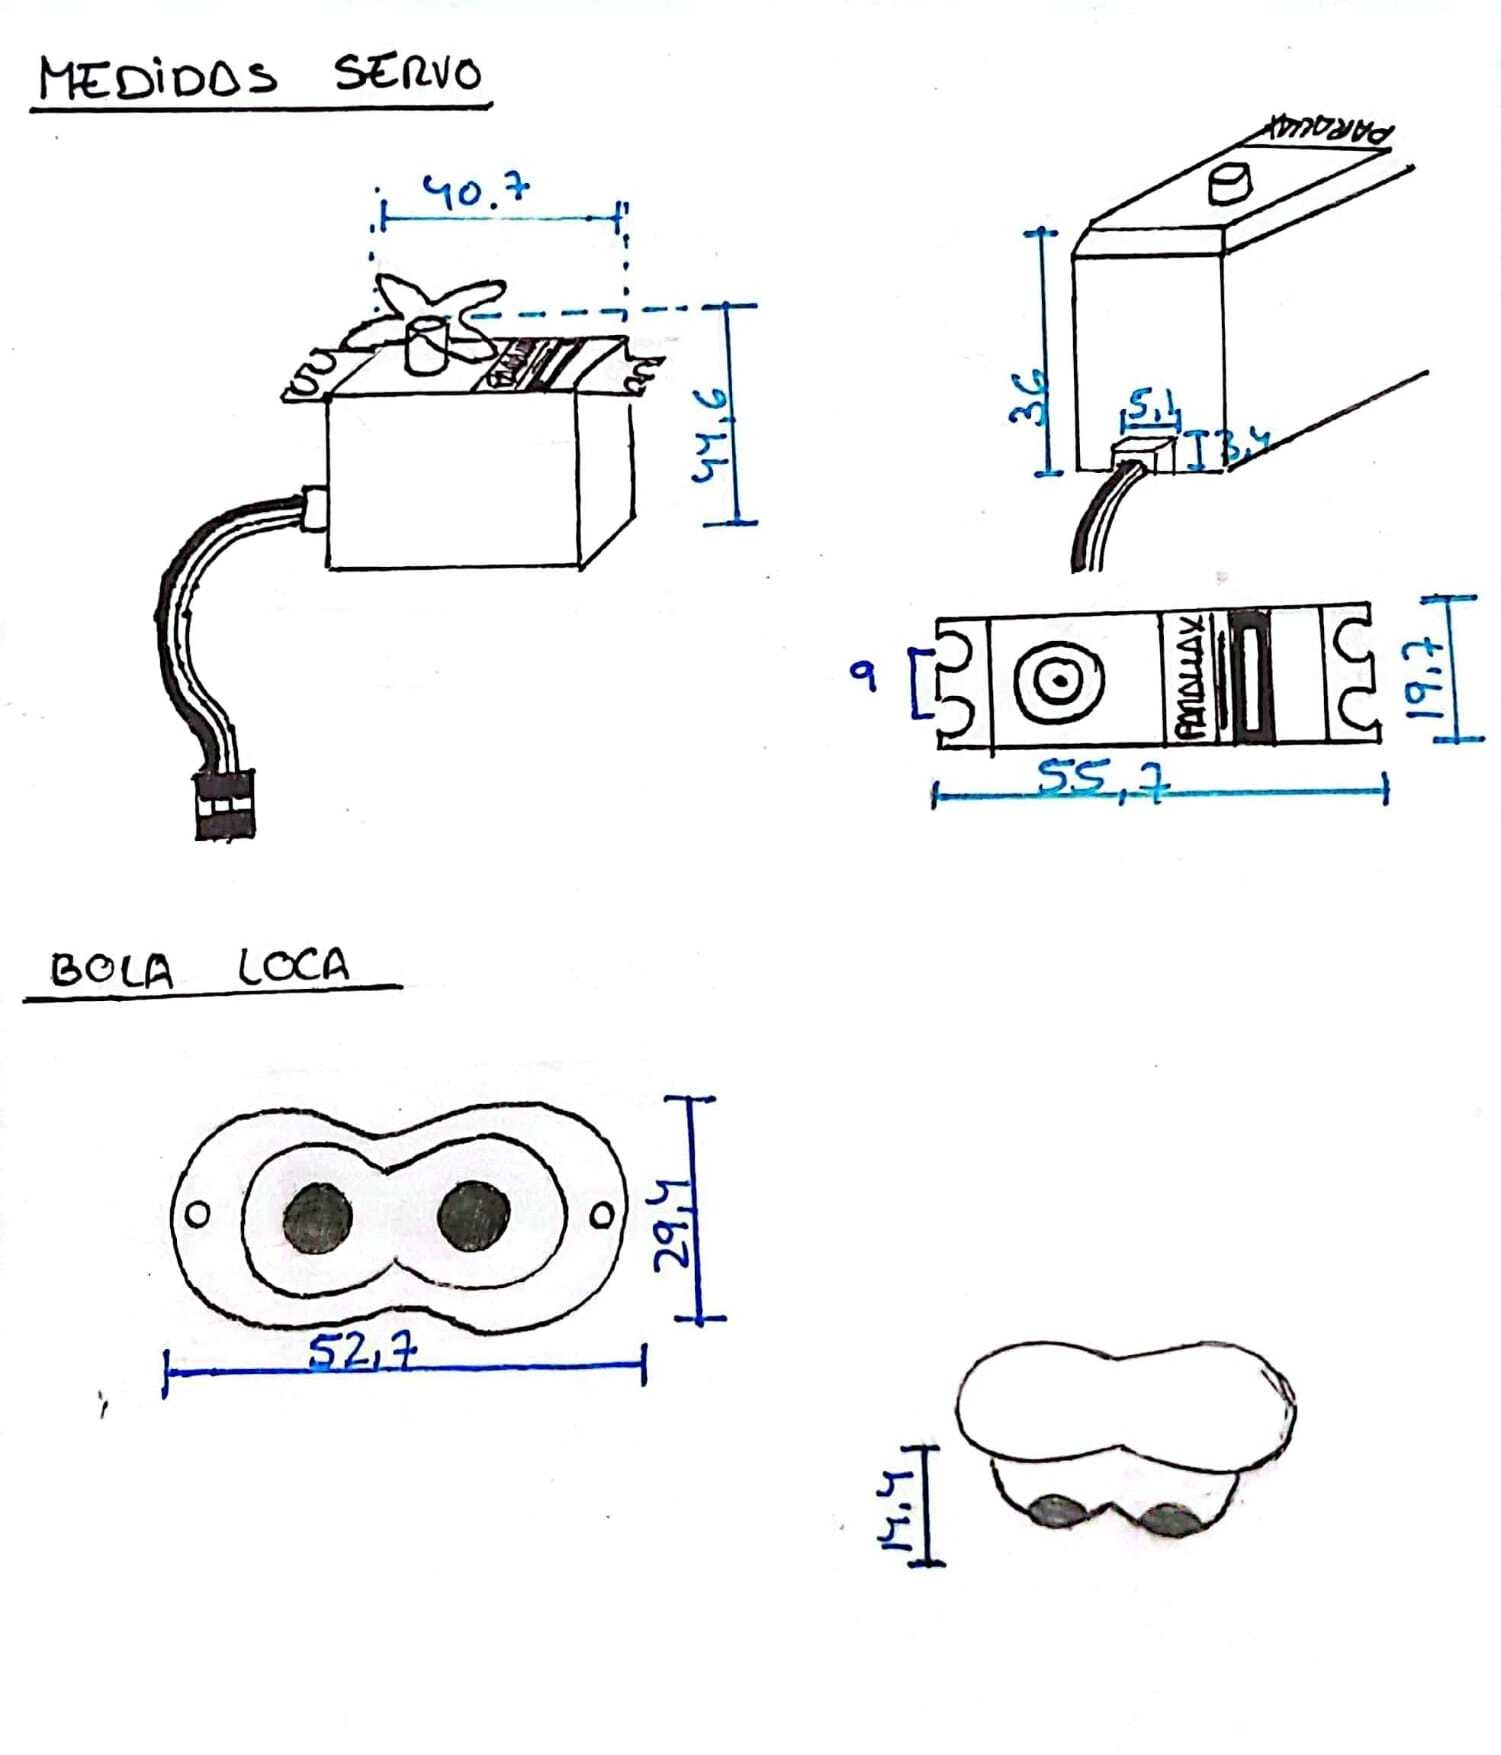
\includegraphics[width=\linewidth]{figs/cap5/planos4.jpeg}
		\caption*{\centering}
	\end{minipage}
	\caption{Planos de los componentes}
	\label{fig:planos}
\end{figure}


%\begin{figure}[ht!]
%	\centering
%	\begin{minipage}{0.4\linewidth}
%		\centering
%		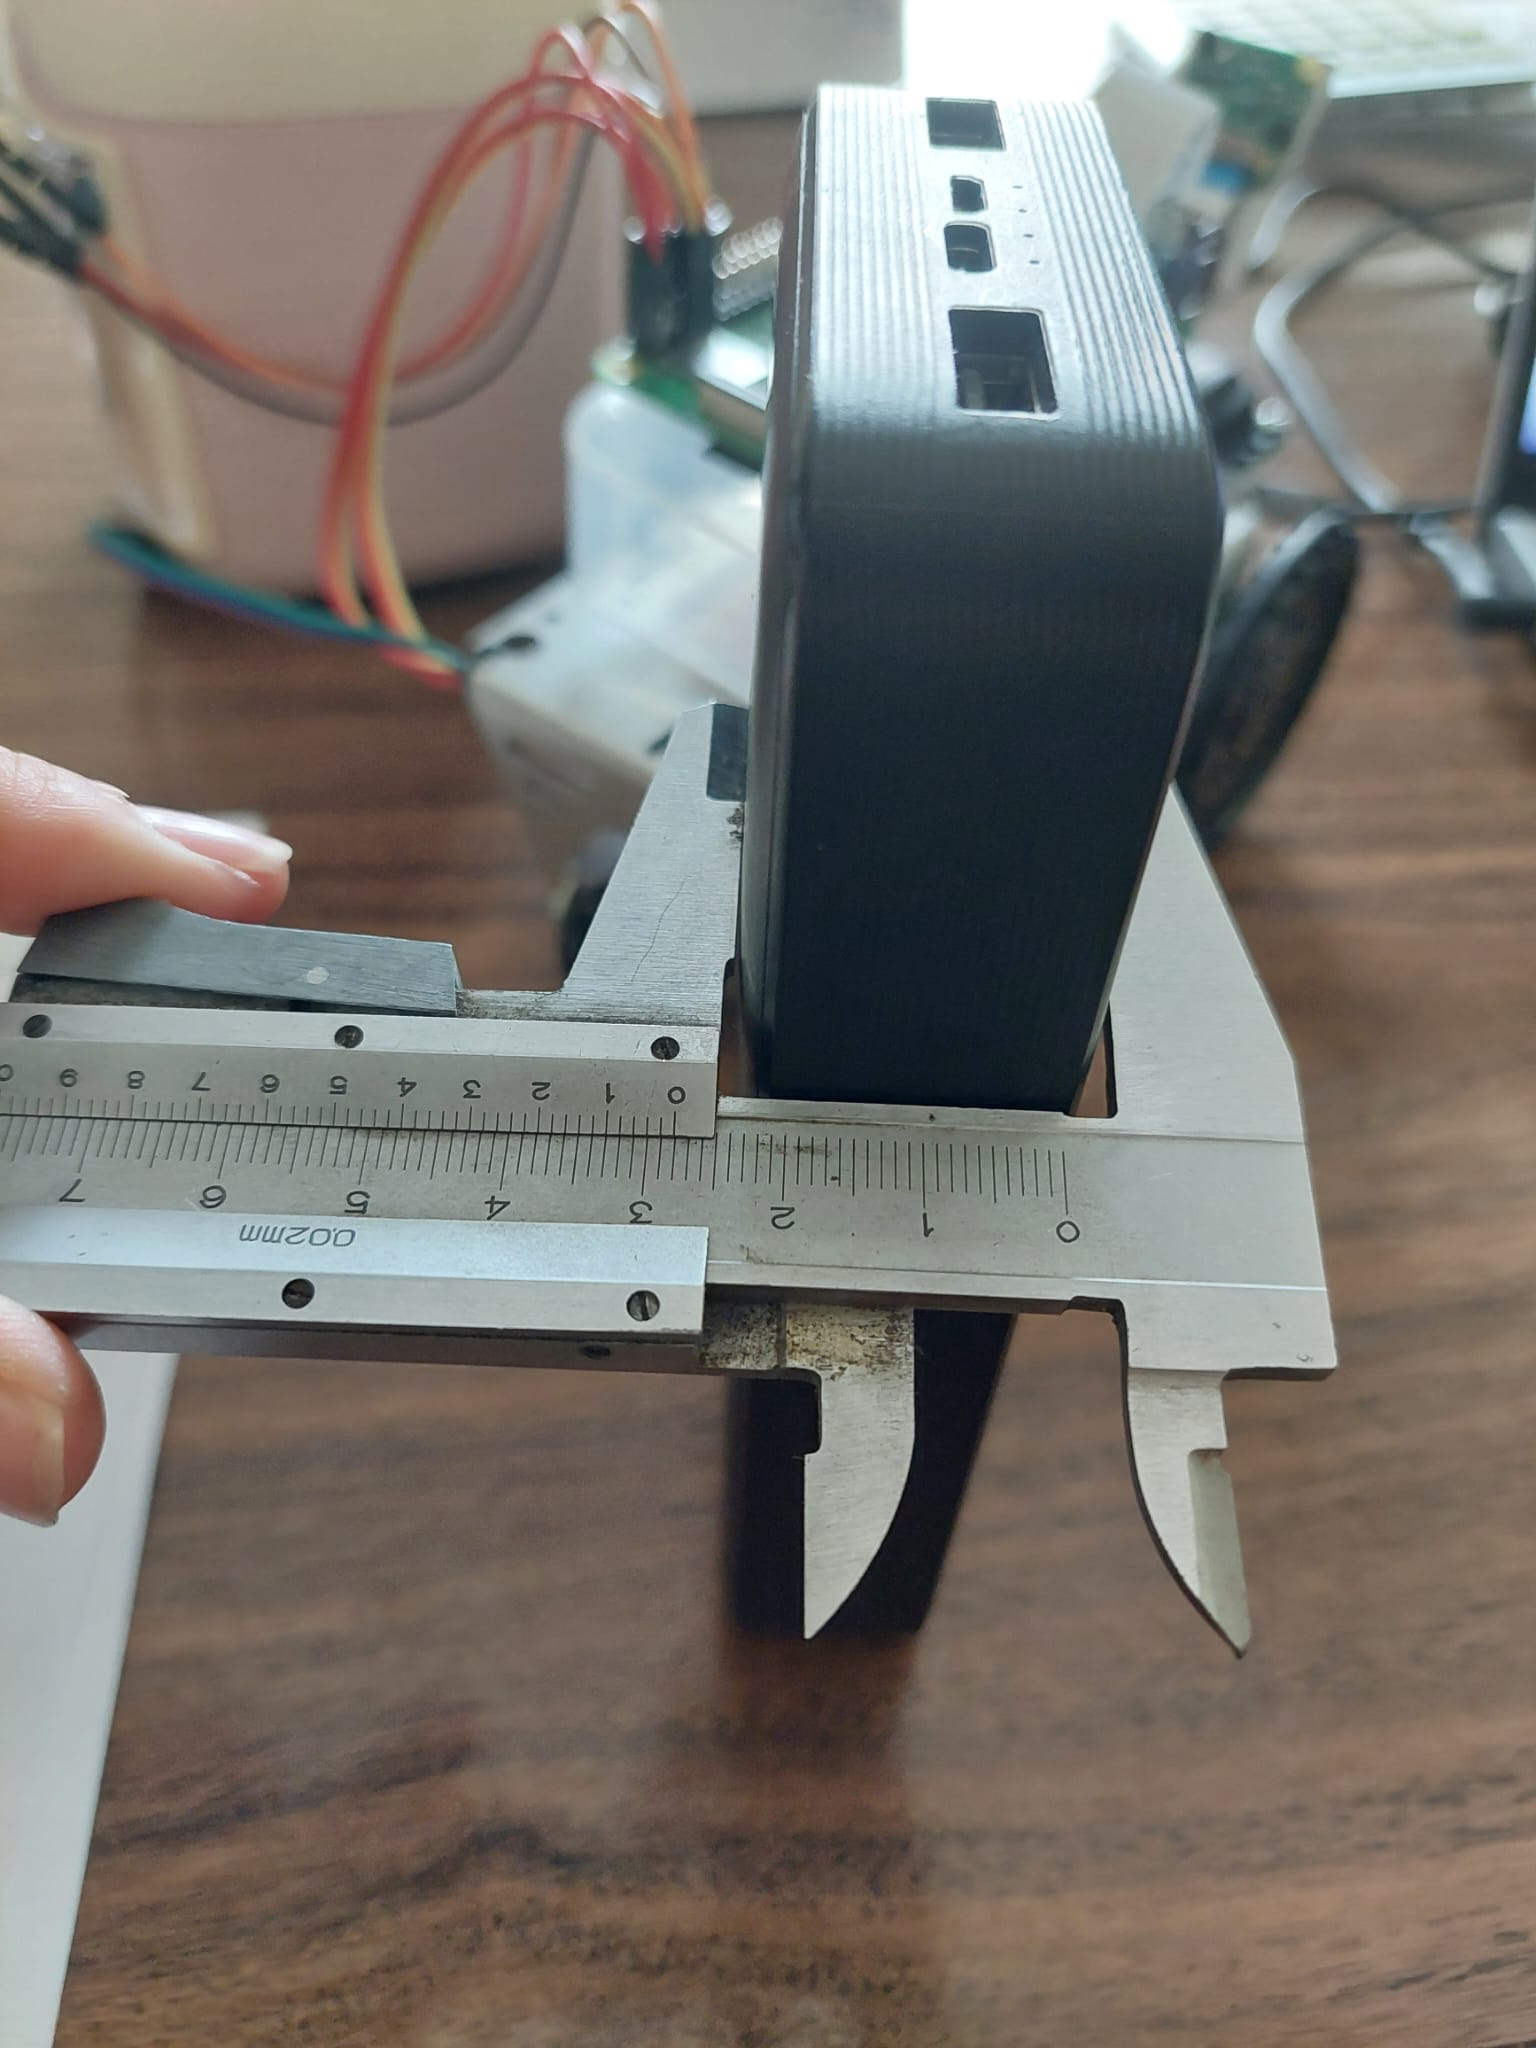
\includegraphics[width=\linewidth]{figs/cap5/calib1.jpeg}
%		\caption*{\centering}
%	\end{minipage}
%	\hspace{2cm}
%	\begin{minipage}{0.4\linewidth}
%		\centering
%		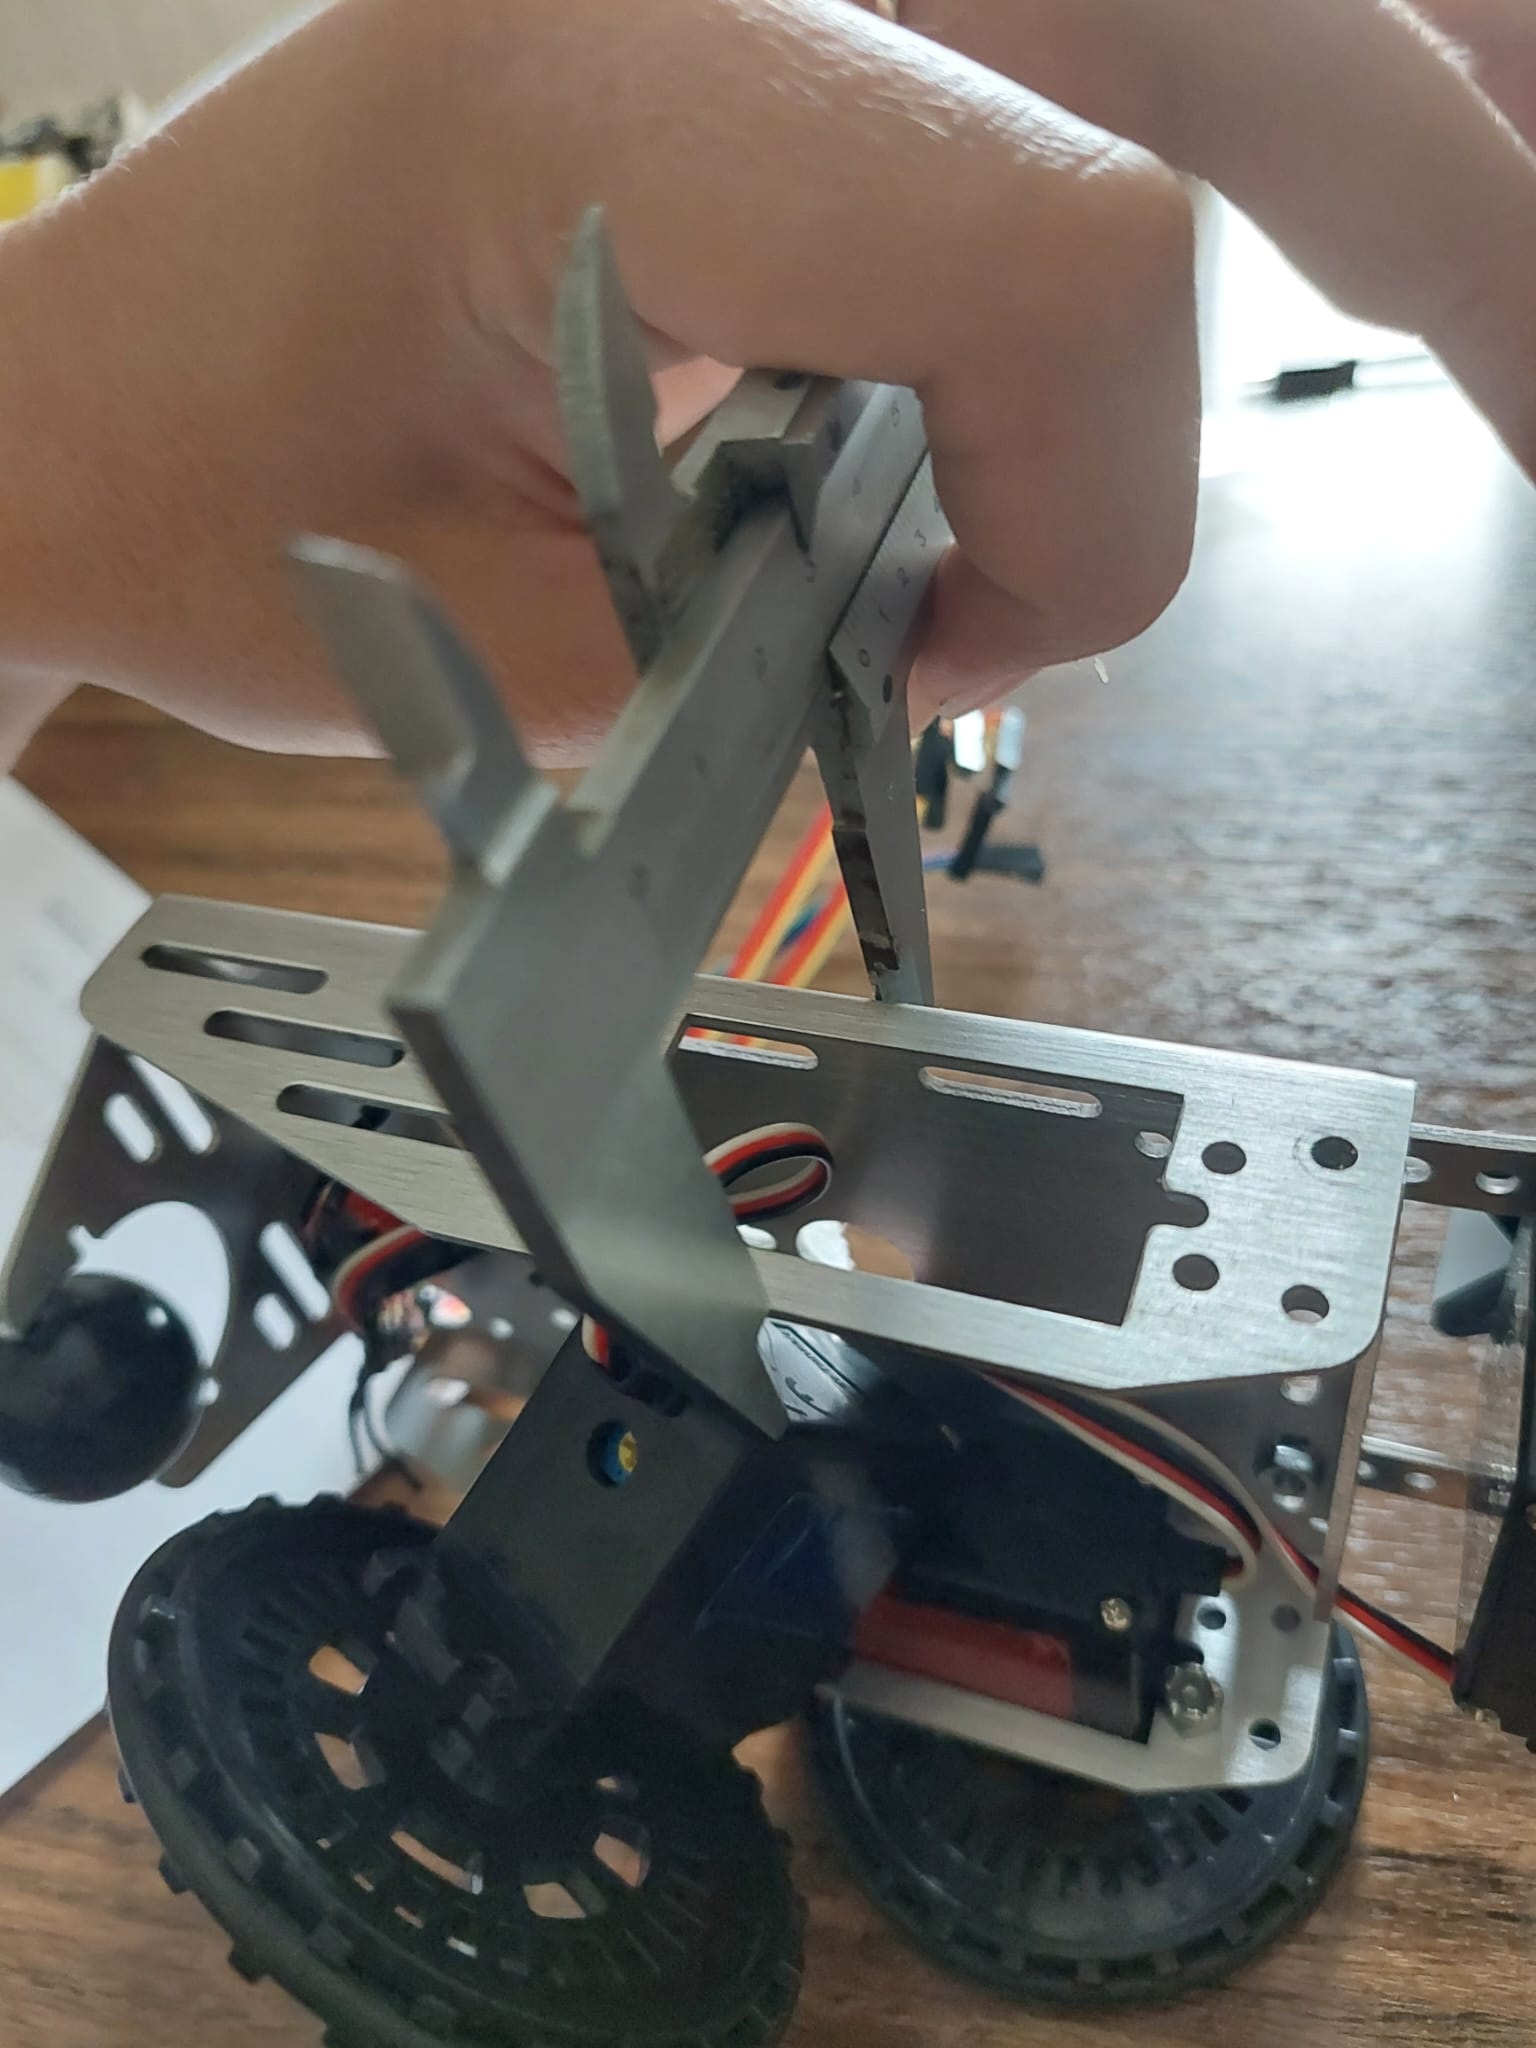
\includegraphics[width=\linewidth]{figs/cap5/calib2.jpeg}
%		\caption*{\centering}
%	\end{minipage}
%	\caption{Comprobación mediante calibre}
%	\label{fig:calibre}
%\end{figure}

\setcounter{footnote}{52}

Para el diseño de PiBotJ se empleó la herramienta de modelado FreeCAD\footnote{\url{https://www.freecad.org/}}, con el objetivo de utilizar \textit{software} libre, permitiendo que cualquier persona pueda acceder y modificar las piezas. El diseño se dividió en cuatro partes, cada una de las cuáles tenía una finalidad específica, descritas a continuación.

Para llevar a cabo el diseño de todas las piezas se han seguido los tutoriales de dos cursos de FreeCAD: el del profesor Juan González (también conocido como \textit{Obijuan})\footnote{\url{https://www.youtube.com/watch?v=2_DbFzFV9D4}}, y el de dcahue-ingeniería\footnote{\url{https://www.youtube.com/watch?v=4zp2DrWv8Wk}}, ambos fundamentales en el desarrollo del proyecto. Además, se han utilizado otros tutoriales específicos, como los dedicados a la creación de \textit{shape binders}\footnote{\url{https://www.youtube.com/watch?v=MCY5IrWrHrU}} y la realización de planos inclinados\footnote{\url{https://www.youtube.com/watch?v=T4hKW1mLrCw}}, esenciales para diseñar la inclinación de la cámara.

\subsection{Chasis}
\label{subsec:chasis}

La estructura principal, que da soporte al robot, fue diseñada para alojar los motores de las ruedas y de la cámara. En la parte trasera se incorporó un prisma rectangular, destinado a la colocación de la rueda loca, mientras que en el lado izquierdo se le dotó con un orificio circular para sujetar la \textit{power bank}. En la parte superior se añadieron seis aberturas rectangulares, para permitir el paso ordenado de los cables, manteniendo una estética limpia y organizada desde el exterior.

Además, a este chasis se le dotó de cuatro orificios circulares, que permitieron fijar la carcasa mediante tornillos. Se puede encontrar tanto su versión compatible con FreeCAD\footnote{\url{https://github.com/RoboticsURJC/tfg-jlopez/blob/main/design/base.FCStd}}, como con el formato de diseño 3D por excelencia, STL\footnote{\url{https://github.com/RoboticsURJC/tfg-jlopez/blob/main/design/base.stl}}. La Figura \ref{fig:pbase} (izquierda) muestra el chasis, tal como será preparada para la impresión en una impresora 3D convencional. Por su parte, la Figura \ref{fig:pbase} (derecha) presenta nuevamente el chasis, pero esta vez equipada con los componentes de \textit{hardware} necesarios.

\begin{figure}[ht!]
	\centering
	\begin{minipage}{0.45\linewidth}
		\centering
		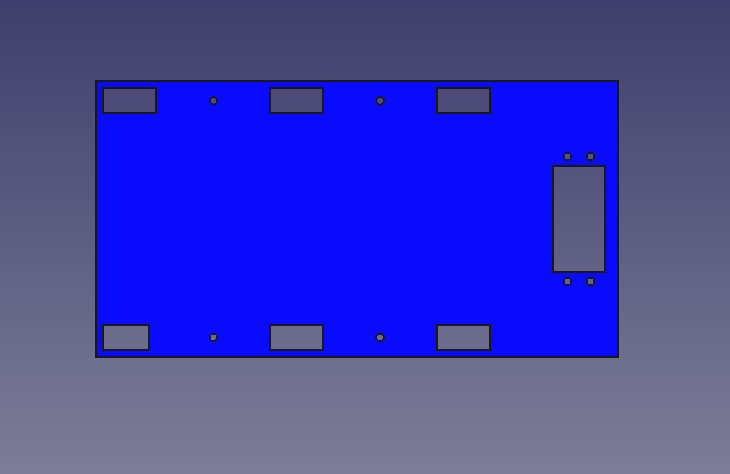
\includegraphics[width=\linewidth]{figs/cap5/basevistasuperiorsin.png}
		%\caption*{\centering} 
	\end{minipage}
	\hspace{1cm}
	\begin{minipage}{0.45\linewidth}
		\centering
		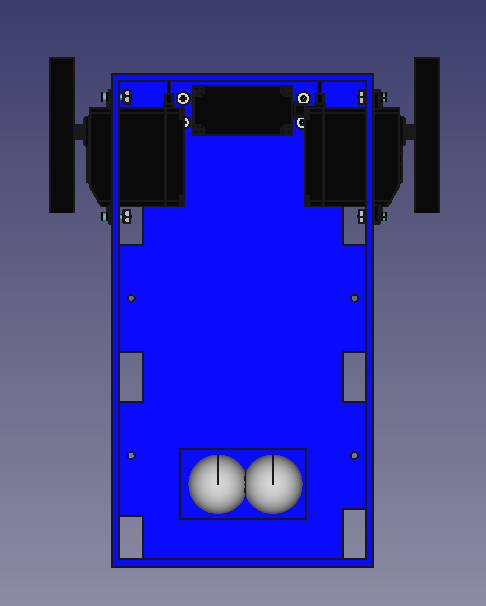
\includegraphics[angle=270, width=\linewidth]{figs/cap5/basecon2.png}
		%\caption*{\centering}
	\end{minipage}
	\caption{Distintas vistas del chasis}
	\label{fig:pbase}
\end{figure}

%\begin{figure}[ht!]
%	\centering
%	\begin{minipage}{0.45\linewidth}
%		\centering
%		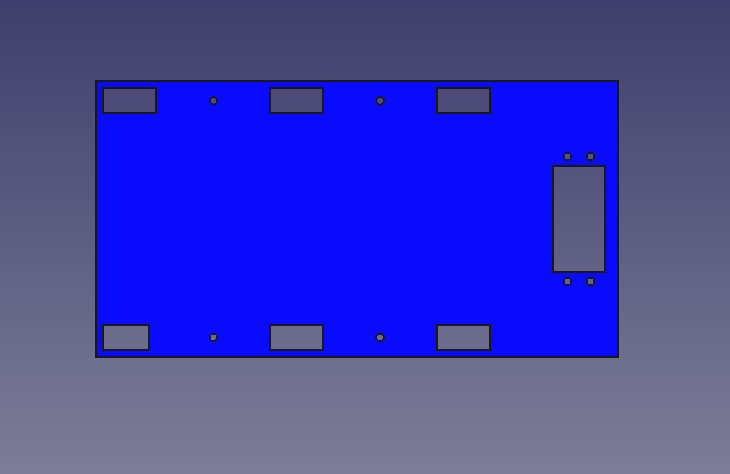
\includegraphics[width=\linewidth]{figs/cap5/basevistasuperiorsin.png}
%		\caption*{\centering} % Vista superior
%	\end{minipage}
%	\hspace{1cm}
%	\begin{minipage}{0.45\linewidth}
%		\centering
%		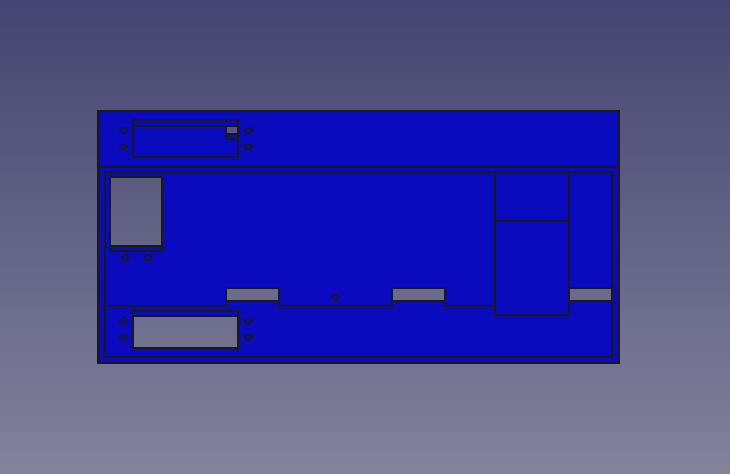
\includegraphics[width=\linewidth]{figs/cap5/basevistaladosin.png}
%		\caption*{\centering} % Vista inferior
%	\end{minipage}
	%\hspace{1cm}
	%\begin{minipage}{0.45\linewidth}
	%	\centering
	%	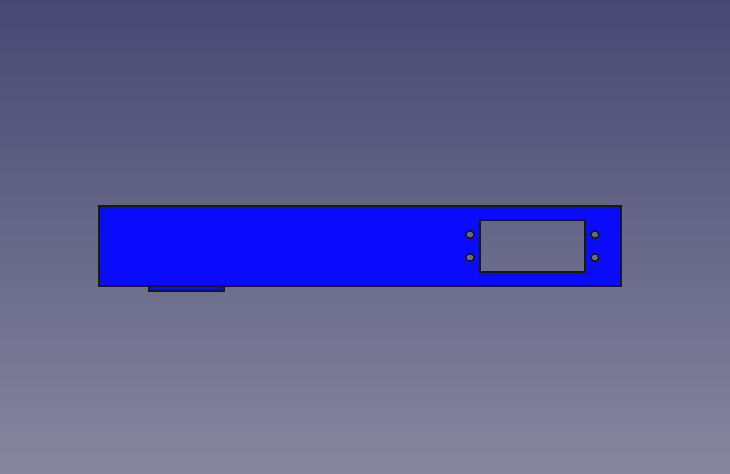
\includegraphics[width=\linewidth]{figs/cap5/basevistalateralsin.png}
	%	\caption*{\centering} % Vista lateral
	%\end{minipage}
	%\hspace{1cm}
	%\begin{minipage}{0.45\linewidth}
	%	\centering
	%	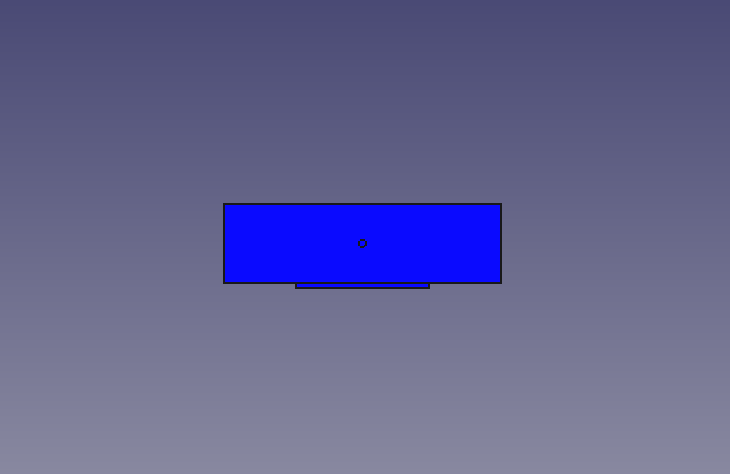
\includegraphics[width=\linewidth]{figs/cap5/basetraserasin.png}
	%	\caption*{\centering} % Vista lateral izquierdo
	%\end{minipage}
	
%	\caption{Distintas vistas del chasis}
%	\label{fig:pbase}
%\end{figure}


%\begin{figure}[ht!]
%	\centering
%	\begin{minipage}{0.45\linewidth}
%		\centering
%		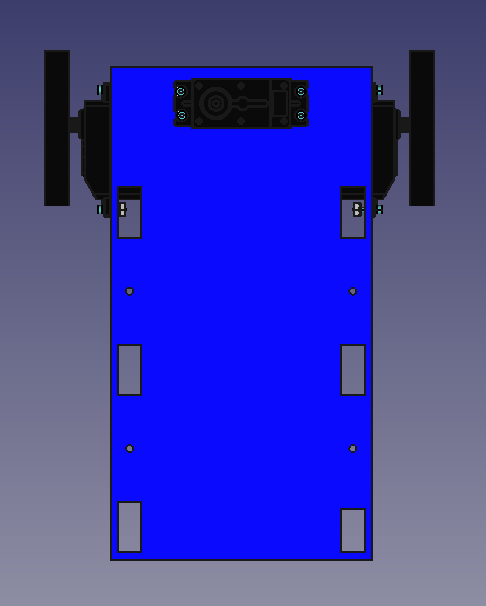
\includegraphics[width=\linewidth]{figs/cap5/basecon1.png}
%		\caption*{\centering}
%	\end{minipage}
%	\hspace{1cm}
%	\begin{minipage}{0.45\linewidth}
%		\centering
%		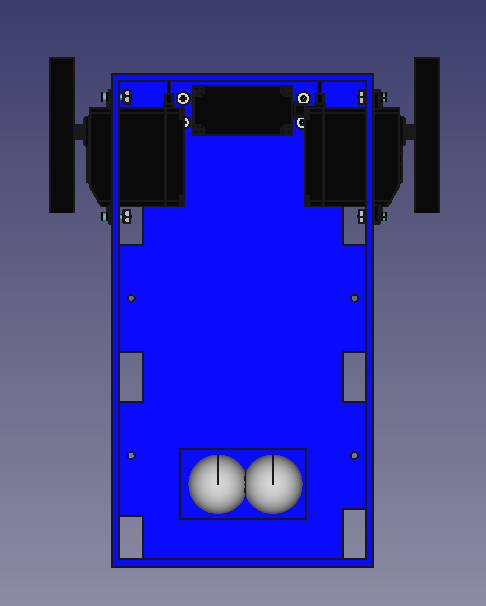
\includegraphics[width=\linewidth]{figs/cap5/basecon2.png}
%		\caption*{\centering}
%	\end{minipage}
%	\caption{Distintas vistas del chasis atornillado}
%	\label{fig:pbasemontada}
%\end{figure}

\subsection{Soporte de la cámara}
\label{subsec:soportecamara}

Para posicionar la cámara de manera que mire hacia el suelo y pueda captar los baches, fue necesario fijarla con una rotación sobre el eje y. En este caso, dicha rotación fue de 50 grados, o 130 grados si se toma como referencia la base de la pieza que va atornillada al motor (Figura \ref{fig:rot}). Esta base fue dotada con dos orificios diagonales que permiten su fijación al motor.

\begin{figure} [h!]
	\begin{center}
		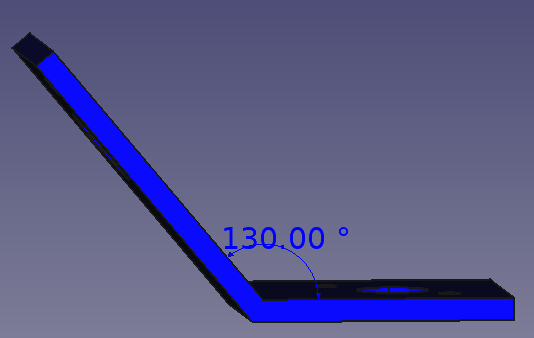
\includegraphics[width=7cm]{figs/cap5/rot.png}
	\end{center}
	\caption{Inclinación de la cámara} 
\label{fig:rot}
\end{figure}

A la parte inclinada de la pieza se le incluyó un orificio diseñado para alojar el sensor CMOS, garantizando una correcta alineación y visión. Además, esta sección fue dotada con dos orificios adicionales para asegurar el sensor CMOS y mantenerlo firmemente en su lugar. Se puede encontrar tanto su versión compatible con FreeCAD\footnote{\url{https://github.com/RoboticsURJC/tfg-jlopez/blob/main/design/camara.FCStd}} como con el formato STL\footnote{\url{https://github.com/RoboticsURJC/tfg-jlopez/blob/main/design/camara.stl}}. La Figura \ref{fig:pcamara} (izquierda) muestra el soporte de la cámara, tal como será preparada para la impresión en una impresora 3D convencional. Por su parte, la Figura \ref{fig:pcamara} (derecha) presenta nuevamente el soporte de la cámara, pero esta vez atornillado sobre los componentes \textit{hardware} necesarios. 

\begin{figure}[ht!]
	\centering
	\begin{minipage}{0.45\linewidth}
		\centering
		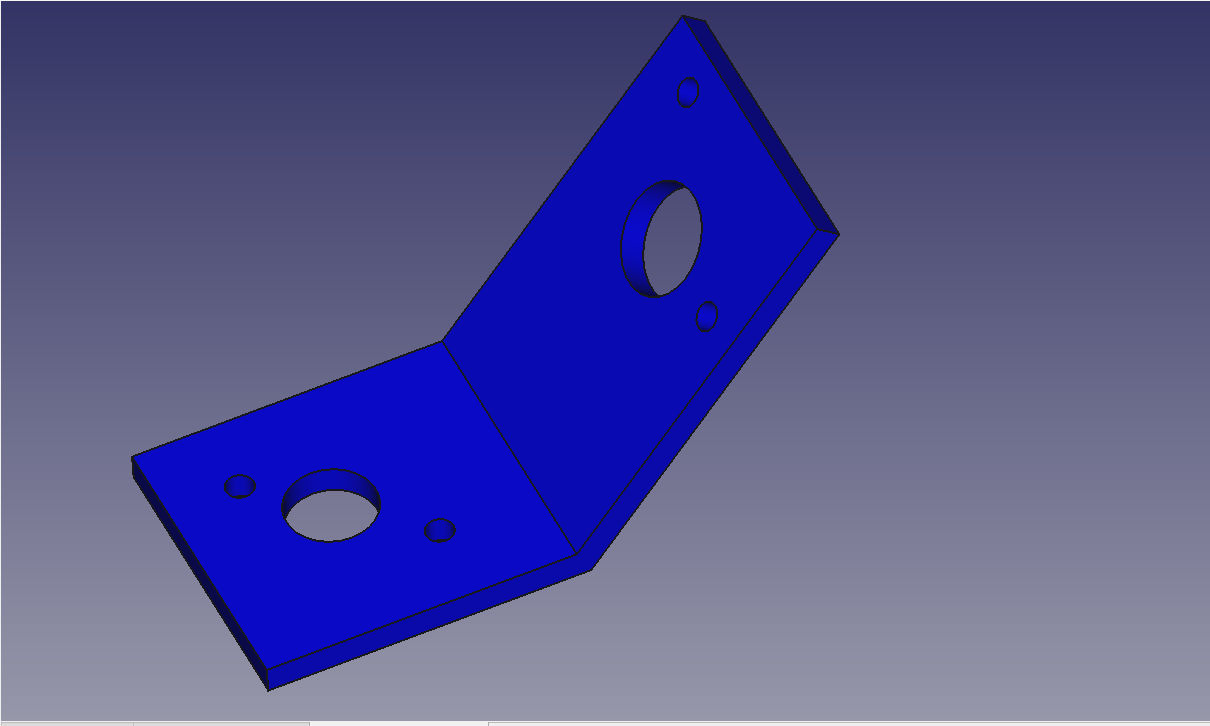
\includegraphics[width=\linewidth]{figs/cap5/camera3sin.png}
		%\caption*{\centering}
	\end{minipage}
	\hspace{1cm}
	\begin{minipage}{0.45\linewidth}
		\centering
		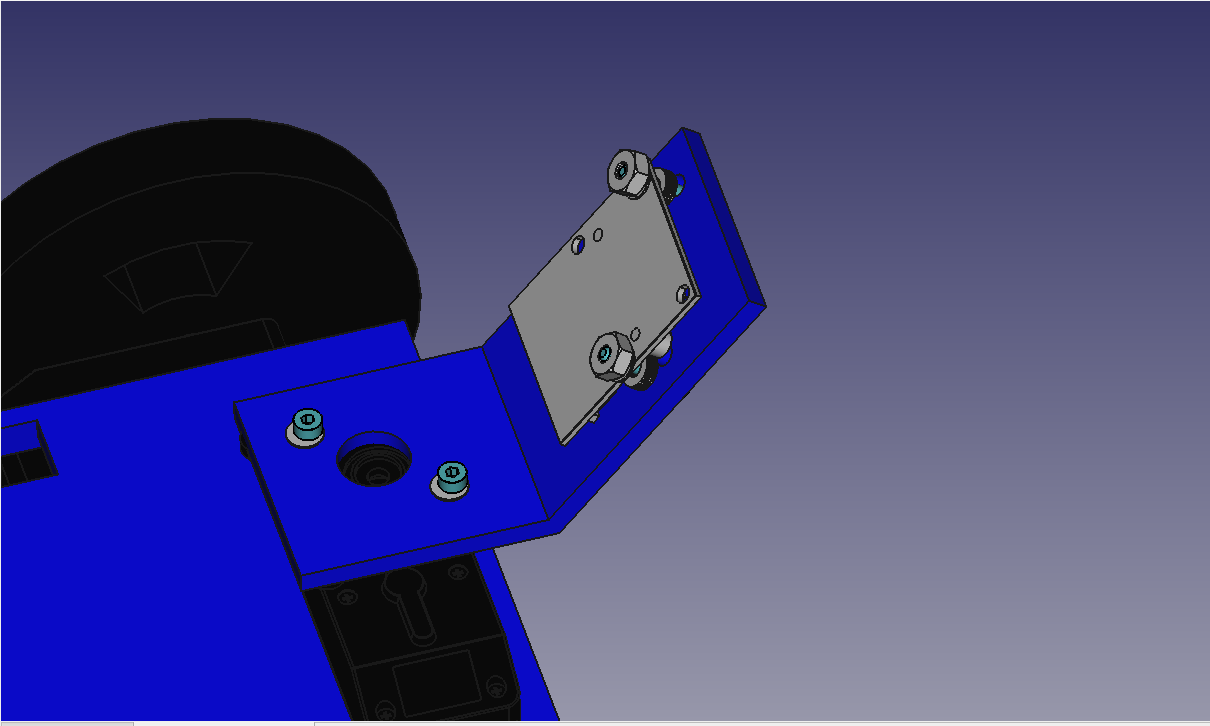
\includegraphics[width=\linewidth]{figs/cap5/camera2con.png}
		%\caption*{\centering}
	\end{minipage}
	\caption{Distintas vistas del soporte de la cámara}
	\label{fig:pcamara}
\end{figure}

%\begin{figure}[ht!]
%	\centering
	%\begin{minipage}{0.45\linewidth}
	%	\centering
	%	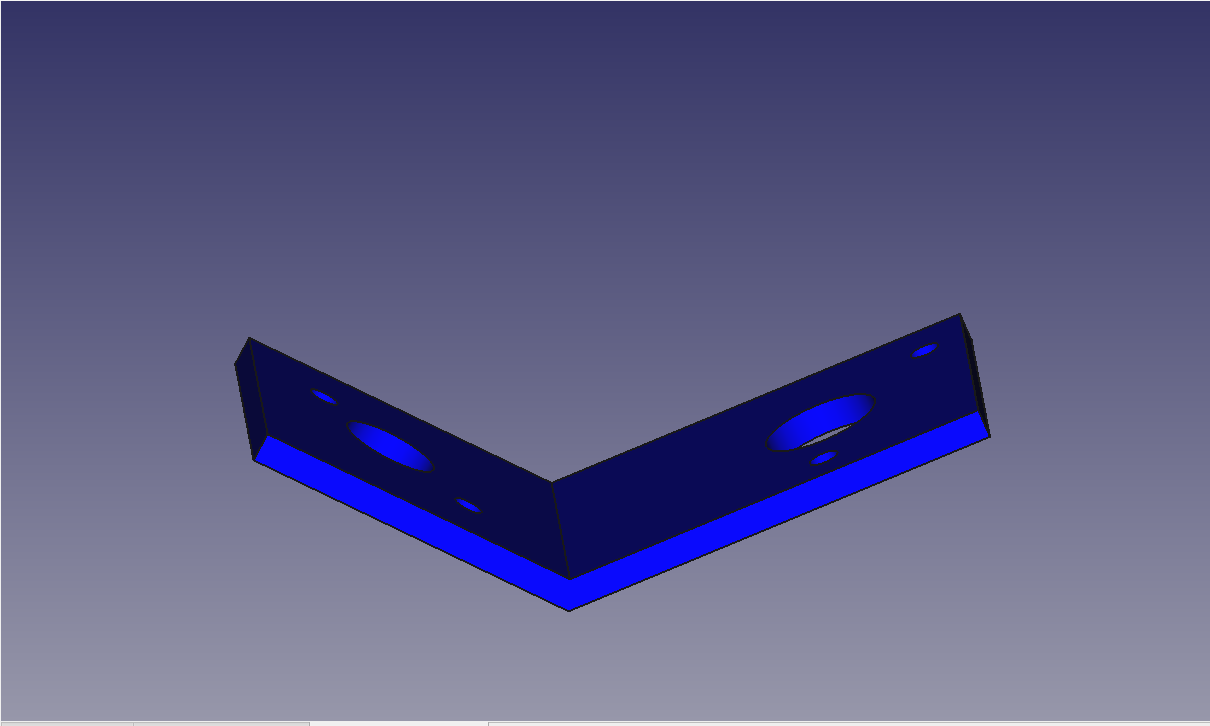
\includegraphics[width=\linewidth]{figs/cap5/camera2sin.png}
	%	\caption*{\centering}
	%\end{minipage}
	%\hspace{1cm}
%	\begin{minipage}{0.45\linewidth}
%		\centering
%		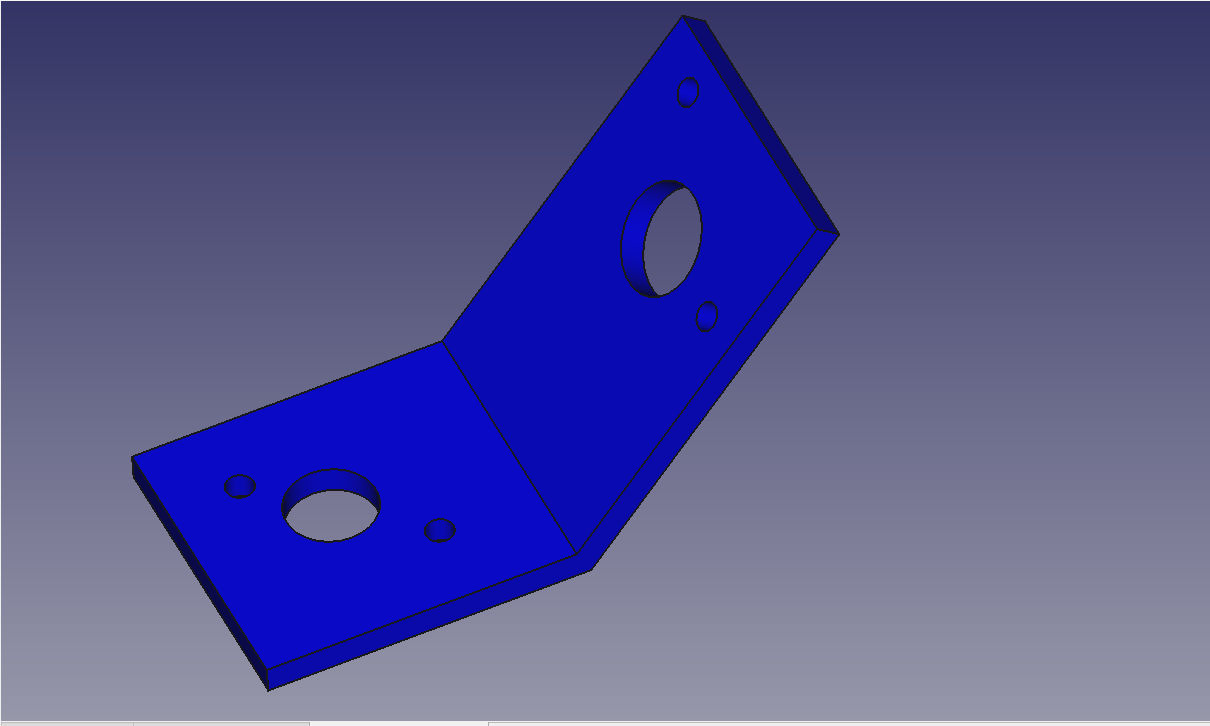
\includegraphics[width=\linewidth]{figs/cap5/camera3sin.png}
%		\caption*{\centering}
%	\end{minipage}
%	\hspace{1cm}
	
	%\caption{Distintas vistas del soporte de la cámara}
	%\label{fig:pcamara}
	%\end{figure}
	
	%\begin{figure}[ht!]
	%\centering
%	\begin{minipage}{0.45\linewidth}
%		\centering
%		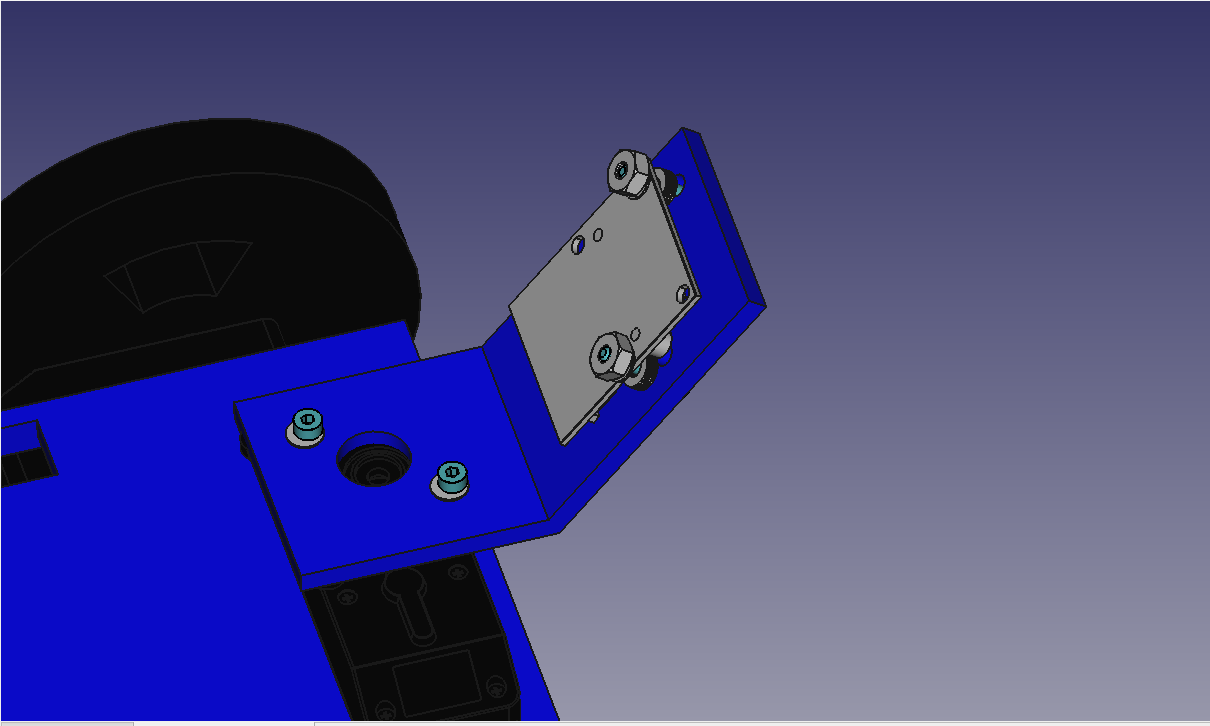
\includegraphics[width=\linewidth]{figs/cap5/camera2con.png}
%		\caption*{\centering}
%	\end{minipage}
	%\hspace{1cm}
	%\begin{minipage}{0.45\linewidth}
	%	\centering
	%	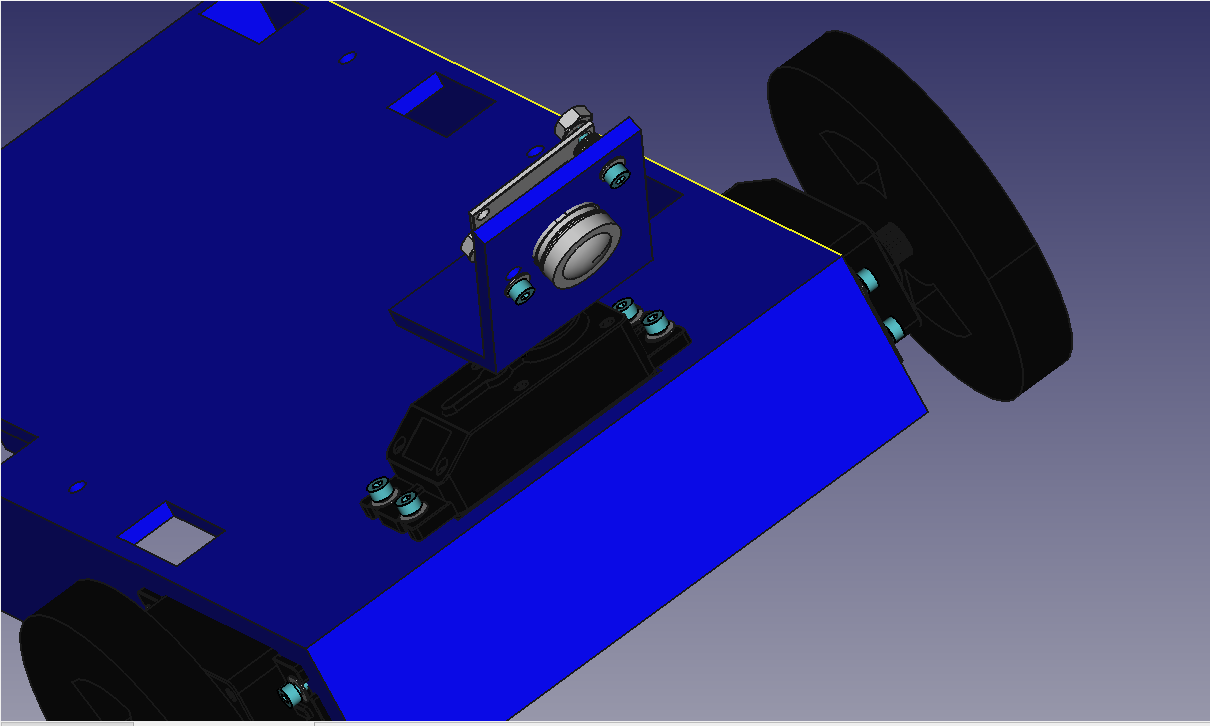
\includegraphics[width=\linewidth]{figs/cap5/camera3con.png}
	%	\caption*{\centering}
	%\end{minipage}
%	\caption{Distintas vistas del soporte de la cámara}
%	\label{fig:pcamara}
%\end{figure}

\subsection{Carcasa}
\label{subsec:carcasa}

Esta carcasa fue diseñada para alojar la placa Raspberry Pi, el módulo GPS y la \textit{power bank} en su interior. La cara superior fue dotada de doce orificios circulares, destinados a atornillar tanto la Raspberry Pi como el módulo GPS, y seis aberturas que se conectaban con la cara inferior, alineándose con las aberturas correspondientes del chasis, para garantizar un paso de cables ordenado.

La cara inferior, además de las seis aberturas, fue dotada con cuatro orificios adicionales para permitir el atornillado del chasis. En el lateral izquierdo, la pieza se dejó abierta para facilitar la inserción de la \textit{power bank}, mientras que en el lado derecho se añadieron dos cuadrantes que permitieron retirar la \textit{power bank} cuando sea necesario. Esta pieza está disponible tanto en formato compatible con FreeCAD\footnote{\url{https://github.com/RoboticsURJC/tfg-jlopez/blob/main/design/parte-superior.FCStd}} como en STL\footnote{\url{https://github.com/RoboticsURJC/tfg-jlopez/blob/main/design/parte-superior.stl}}.

La Figura \ref{fig:psuperior} (izquierda) muestra la carcasa, lista para la impresión en una impresora 3D convencional. La Figura \ref{fig:psuperior} (derecha) presenta nuevamente la carcasa, pero equipada con los componentes \textit{hardware} necesarios.


%\begin{figure}[ht!]
%	\centering
%	\begin{minipage}{0.45\linewidth}
%		\centering
%		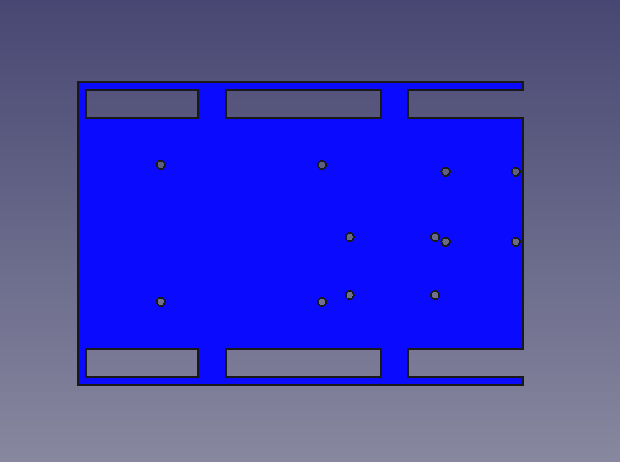
\includegraphics[width=\linewidth]{figs/cap5/superior1.png}
%		\caption*{\centering} % vista superior 
%	\end{minipage}
%	\hspace{1cm}
%	\begin{minipage}{0.45\linewidth}
%		\centering
%		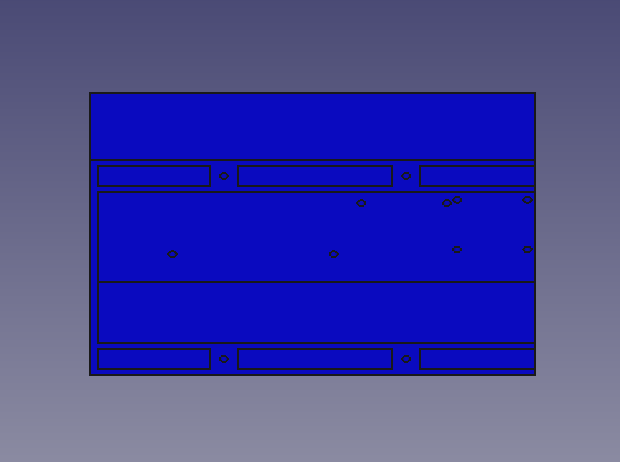
\includegraphics[width=\linewidth]{figs/cap5/superior2.png}
%		\caption*{\centering} % vista inferior
%	\end{minipage}
%	\hspace{1cm}
%	\begin{minipage}{0.45\linewidth}
%		\centering
%		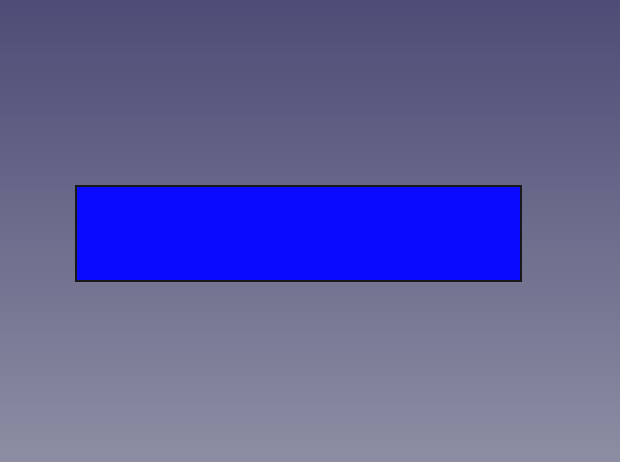
\includegraphics[width=\linewidth]{figs/cap5/superior3.png}
%		\caption*{\centering}  % vista lateral 
%	\end{minipage}
%	\hspace{1cm}
%	\begin{minipage}{0.45\linewidth}
%		\centering
%		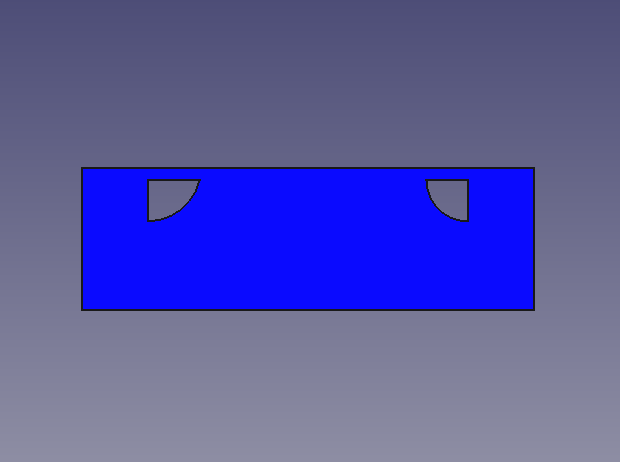
\includegraphics[width=\linewidth]{figs/cap5/superior4.png}
%		\caption*{\centering} % vista lateral izquierdo
%	\end{minipage}
	
%	\caption{Distintas vistas de la carcasa}
%	\label{fig:psuperior}
%\end{figure}


%\begin{figure}[ht!]
%	\centering
%	\begin{minipage}{0.45\linewidth}
%		\centering
%		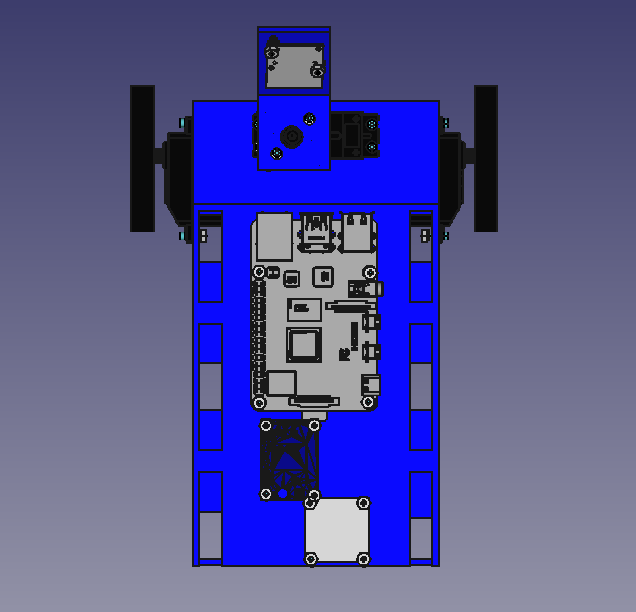
\includegraphics[width=\linewidth]{figs/cap5/superior1m.png}
%		\caption*{\centering}
%	\end{minipage}
%	\hspace{1cm}
%	\begin{minipage}{0.45\linewidth}
%		\centering
%		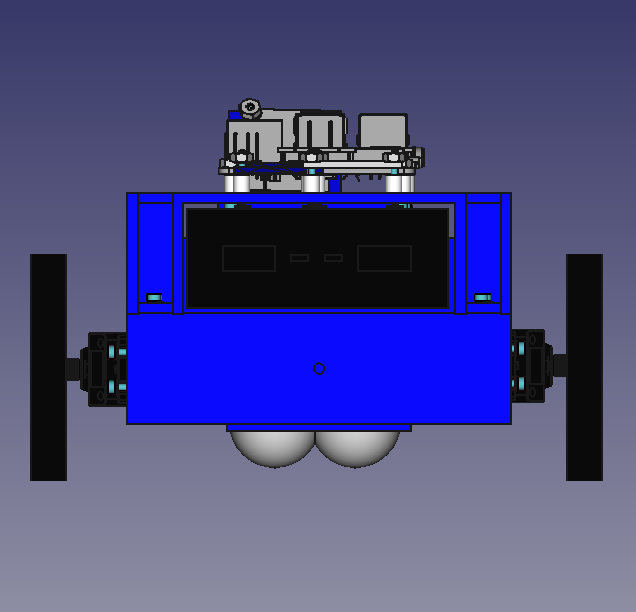
\includegraphics[width=\linewidth]{figs/cap5/superior2m.png}
%		\caption*{\centering}
%	\end{minipage}
%	\caption{Distintas vistas de la carcasa atornillada}
%	\label{fig:psuperiormontada}
%\end{figure}

\begin{figure}[ht!]
	\centering
	\begin{minipage}{0.46\linewidth}
		\centering
		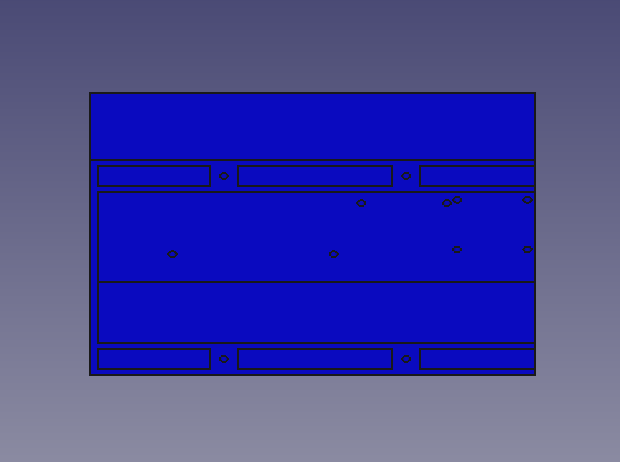
\includegraphics[width=\linewidth]{figs/cap5/superior2.png}
		%\caption*{\centering}
	\end{minipage}
	\hspace{1cm}
	\begin{minipage}{0.45\linewidth}
		\centering
		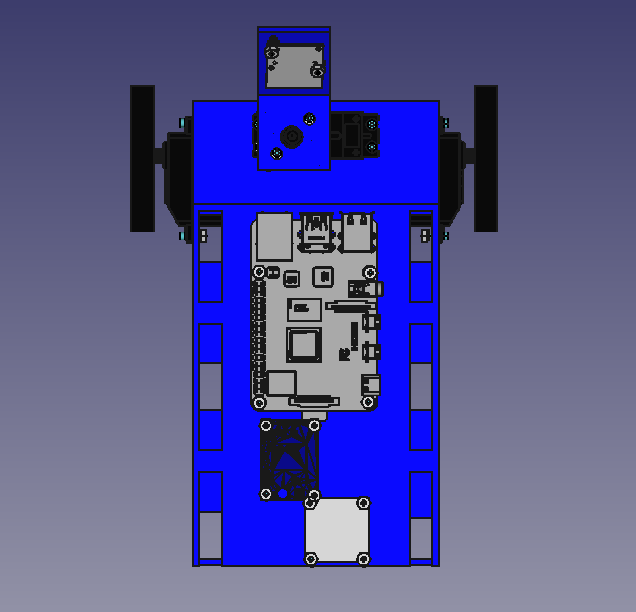
\includegraphics[angle=270, width=\linewidth]{figs/cap5/superior1m.png}
		%\caption*{\centering}
	\end{minipage}
	\caption{Distintas vistas de la carcasa}
	\label{fig:psuperior}
\end{figure}


\subsection{Sujección trasera}
\label{subsec:sujecciontrasera}

Para asegurar que la \textit{power bank} se mantenga en su lugar dentro del robot, se diseñó una pieza que se atornilla en el lado izquierdo del chasis. Esta pieza fue definida como un prisma rectangular con más de 30 mm de altura, aproximadamente 5 mm de largo y 3 mm de ancho (Figura \ref{fig:ptrasera} izquierda). La pieza debe colocarse en posición vertical para evitar que la \textit{power bank} se deslice, y en posición horizontal cuando se desea extraer esta. Existe una versión en FreeCAD\footnote{\url{https://github.com/RoboticsURJC/tfg-jlopez/blob/main/design/sujeccion-trasera.FCStd}} y otra en formato STL\footnote{\url{https://github.com/RoboticsURJC/tfg-jlopez/blob/main/design/sujeccion-trasera.stl}}. La Figura \ref{fig:ptrasera} (derecha) muesta cómo quedaría montada la pieza sobre el robot.

%\begin{figure}[ht!]
%	\centering
%	\begin{minipage}{0.45\linewidth}
%		\centering
%		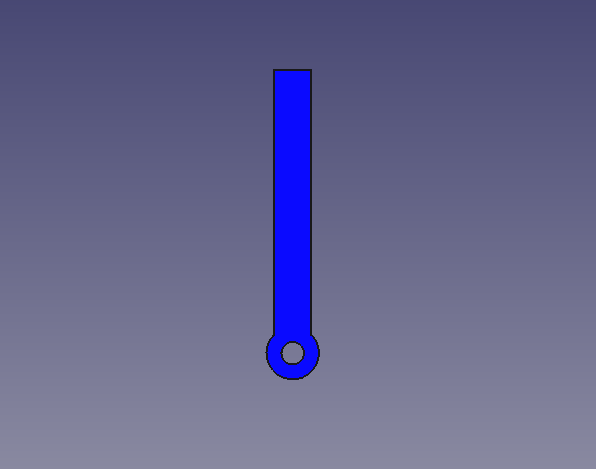
\includegraphics[width=\linewidth]{figs/cap5/trasera1.png}
%		\caption*{\centering}
%	\end{minipage}
%	\hspace{1cm}
%	\begin{minipage}{0.45\linewidth}
%		\centering
%		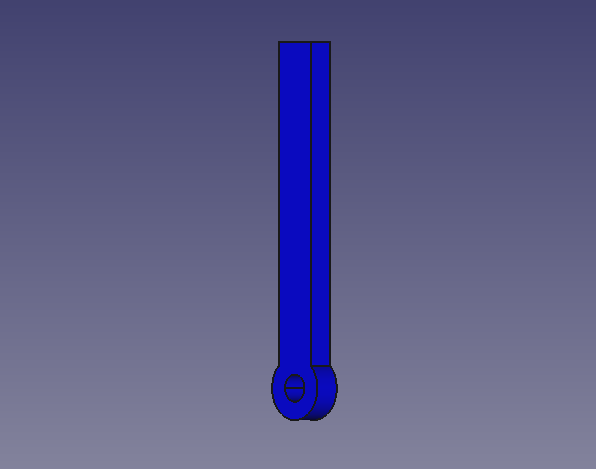
\includegraphics[width=\linewidth]{figs/cap5/trasera2.png}
%		\caption*{\centering}
%	\end{minipage}
%	\caption{Distintas vistas de la pieza para la sujección trasera}
%	\label{fig:ptrasera}
%\end{figure}

%\begin{figure} [h!]
%	\begin{center}
%		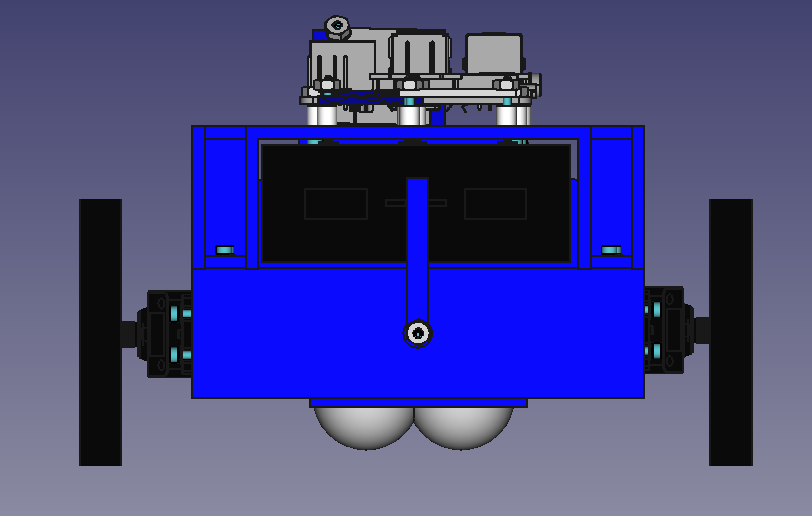
\includegraphics[width=8cm]{figs/cap5/traseracon.png}
%	\end{center}
%	\caption{Pieza para la sujección trasera atornillada} 
%	\label{fig:traseracon}
%\end{figure}

\begin{figure}[ht!]
	\centering
	\begin{minipage}{0.365\linewidth}
		\centering
		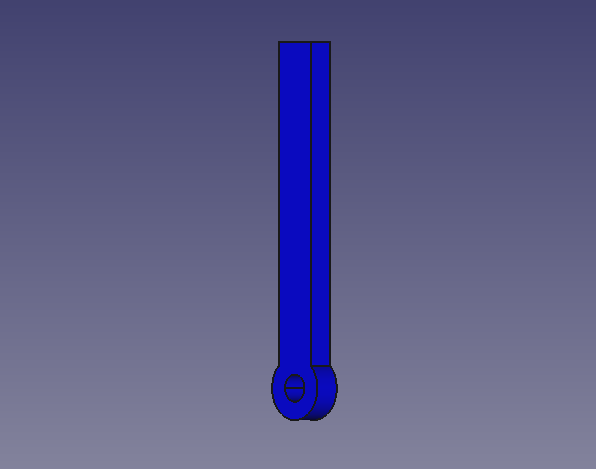
\includegraphics[width=\linewidth]{figs/cap5/trasera2.png}
		%\caption*{\centering}
	\end{minipage}
	\hspace{1cm}
	\begin{minipage}{0.45\linewidth}
		\centering
		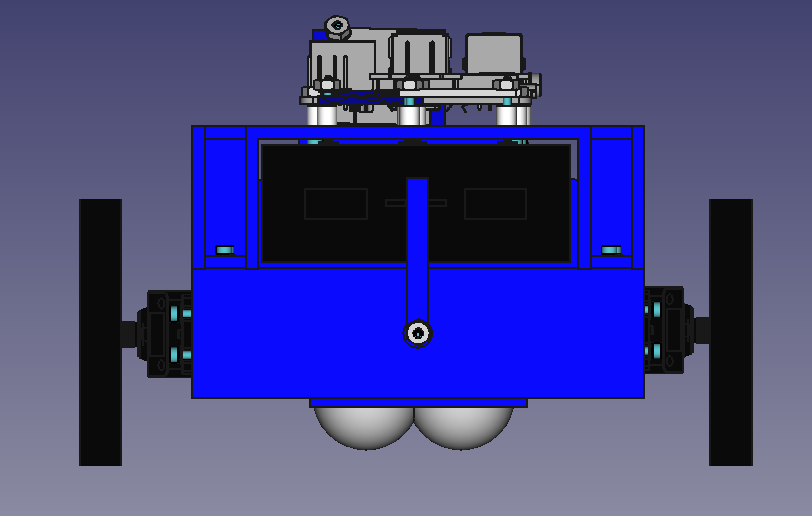
\includegraphics[width=\linewidth]{figs/cap5/traseracon.png}
		%\caption*{\centering}
	\end{minipage}
	\caption{Distintas vistas de la pieza para la sujección trasera}
	\label{fig:ptrasera}
\end{figure}

Una vez detalladas cada una de las piezas \acs{CAD} diseñadas, se continúa describiendo el proceso de impresión y montaje que se ha seguido para conseguir finalmente el prototipo robótico PiBotJ.
  
\section{Impresión y montaje}
\label{sec:impresionmontaje}

En esta sección se presentan todos los detalles que deben considerarse para replicar este proyecto mediante impresión 3D. 

En nuestro caso, para la impresión de PiBotJ, se usó la impresora FDM Creality Ender3 V2 (Figura \ref{fig:impresora}), un rollo de PLA convencional azul y Ultimaker Cura\footnote{\url{https://ultimaker.com/es/software/ultimaker-cura/}} como \textit{software} de impresión. Para la impresión de todas las piezas se emplearon las mismas características que muestra el Cuadro \ref{cuadro:cimpresion}. Para este proyecto fue necesario imprimir una pieza de cada una de las explicadas en el apartado de Diseño CAD (Sección \ref{sec:diseñocad}), como muestra la Figura \ref{fig:piezasimpresas}. La duración de impresión fue en torno a 50 horas.
 
\begin{figure} [h!]
	\begin{center}
		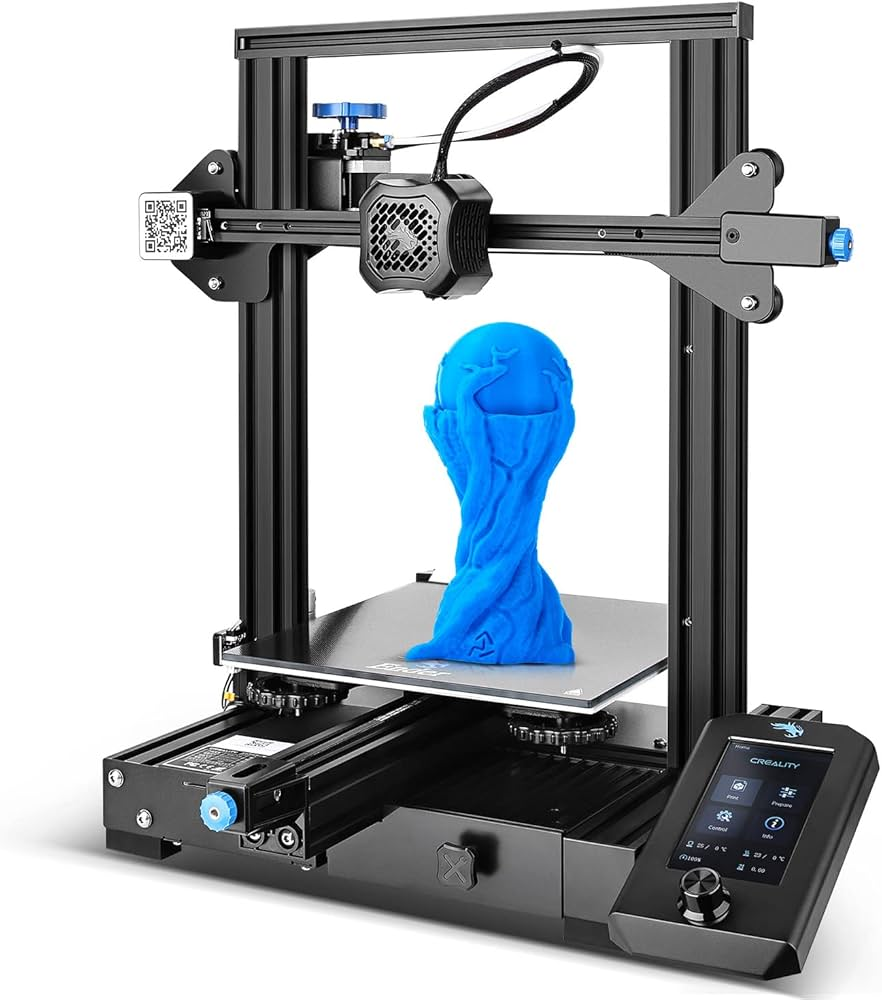
\includegraphics[width=6cm]{figs/cap5/impresora.jpg}
	\end{center}
	\caption{Impresora FDM Creality Ender3 V2$^{\ref{note:enlace67}}$} 
	\label{fig:impresora}
\end{figure}

\setcounter{footnote}{67} % Establecer la numeración de la siguiente nota al pie
\footnotetext[\value{footnote}]{\url{https://www.creality.com/es/products/ender-3-v2-neo-3d-printer}\label{note:enlace67}}

\begin{table}[H]
	\begin{center}
		\begin{tabular}{|c|c|}
			\hline
			Características & Parámetros\\
			\hline
			\multirow{2}{*}{Calidad} & \multirow{2}{*}{\shortstack{ Altura de capa: 0,2 mm \\ Ancho de línea: 0,4 mm}}\\
			& \\
			\hline
			\multirow{4}{*}{Paredes} & \multirow{4}{*}{\shortstack{Grosor de pared: 0,8 mm \\ Cantidad de líneas de pared: 2 \\ Alineación de costura en Z: \textit{Esquina más afilada} \\ Preferencia de costura en esquina: \textit{Ocultación inteligente} }} \\
			& \\
			& \\
			& \\
			\hline
			
			\multirow{2}{*}{\shortstack{Relleno}} &  \multirow{2}{*}{\shortstack{Densidad de relleno: 15\% \\ Patrón de relleno: \textit{Gyroid} }}\\
			& \\
			\hline
			\multirow{2}{*}{\shortstack{Velocidad}} &  \multirow{2}{*}{\shortstack{Velocidad de impresión: 50 mm/s\\ Velocidad de la primera capa: 20 mm/s}}\\
			& \\
			\hline
		\end{tabular}
		\caption{Características usadas para la impresión}
		\label{cuadro:cimpresion}
	\end{center}
\end{table}


\begin{figure} [h!]
	\begin{center}
		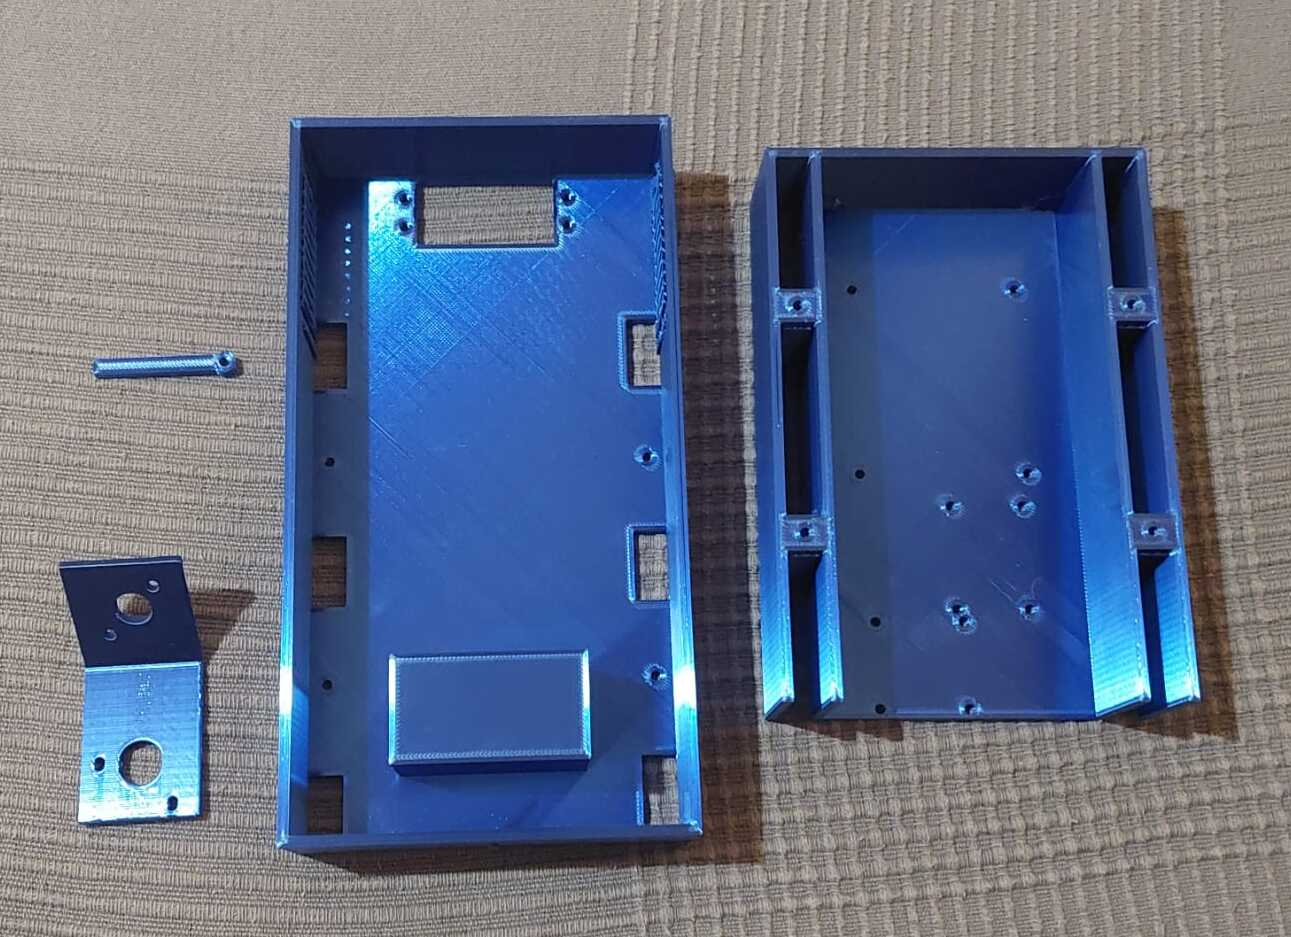
\includegraphics[width=10cm]{figs/cap5/setcompleto.jpeg}
	\end{center}
	\caption{Piezas impresas} 
	\label{fig:piezasimpresas}
\end{figure}


Una vez impresas todas las piezas y retirados sus soportes generados, fue el momento del montaje, cuya duración fue de dos horas aproximadamente, pero puede ser más dependiendo de las habilidades del usuario.

Uno de los elementos que se tuvo que tener en cuenta para el montaje fueron los Hama Beads\footnote{\url{https://www.hamabeads.es/}}. Los Hama Beads son cilindros de plástico pequeños con un círculo en el centro usados comunmente para manualidades y para la creación de objetos de decoración. En este caso, se usaron para evitar que tanto la Raspberry Pi como el módulo GPS toquen directamente la superficie impresa. Además, por su círculo interior pasaban perfectamente los tornillos usados. 

%Uno de los elementos que se tuvo que tener en cuenta para el montaje fueron los Hama Beads (Figura \ref{fig:hamabeads}). Los Hama Beads son cilindros de plástico pequeños con un círculo en el centro usados comunmente para manualidades y para la creación de objetos de decoración. En este caso, se usaron para evitar que tanto la Raspberry Pi como el módulo GPS toquen directamente la superficie impresa. Además, por su círculo interior pasaban perfectamente los tornillos usados. 

%\begin{figure} [h!]
%	\begin{center}
%		\includegraphics[width=6cm]{figs/cap5/hama.png}
%	\end{center}
%	\caption{Hama Beads$^{\ref{note:enlace80}}$} 
%	\label{fig:hamabeads}
%\end{figure}

%\setcounter{footnote}{80} % Establecer la numeración de la siguiente nota al pie
%\footnotetext[\value{footnote}]{\url{https://www.hamabeads.es/}\label{note:enlace80}}


Otro aspecto a tener en cuenta es que, para la placa del módulo GPS, fue necesario soldarle unos pines (Figura \ref{fig:soldar}) para posteriormente conectarle los cables sin pérdidas de señal. También fue necesario agrandar con una taladradora los cuatro agujeros que tiene la antena del módulo para que puedan entrar bien los tornillos. 

\begin{figure} [h!]
	\begin{center}
		\includegraphics[width=7cm]{figs/cap5/soldar.jpeg}
	\end{center}
	\caption{Soldando pines al módulo GPS} 
	\label{fig:soldar}
\end{figure}

Una vez solventados los contratiempo anteriores, se puede pasar a la fase de fijación de piezas mediante tornillos. El Cuadro \ref{cuadro:tornillos} muestra toda la tornillería necesaria.Los tornillos, tuercas y arandelas se pueden obtener en cualquier ferretería. Se recomienda usar un fijador para evitar que se aflojen los tornillos.

Se ha creado en FreeCAD\footnote{\url{https://github.com/RoboticsURJC/tfg-jlopez/blob/main/design/robotcompleto.FCStd}}, un diseño de PiBotJ completo, que muestra el lugar donde se sitúa la tornillería del robot y ayudará al usuario facilitar el ensamblaje. La Figura \ref{fig:robotfreecad} muestra el robot completo montado. Para conseguir realizar el diseño de PiBotJ completo en FreeCAD, se tomaron los ficheros .stl obtenidos de la Sección \ref{sec:diseñocad}. Además, se tuvo que diseñar aparte: la antena del módulo \acs{GPS}, la batería, la rueda loca, un Hama Bead y la rueda; todos los ficheros se pueden encontrar en la carpeta \verb|misc|\footnote{\url{https://github.com/RoboticsURJC/tfg-jlopez/tree/main/design/misc}}. La placa del módulo \acs{GPS} necesitó ser editada partiendo de una versión de Thinkercad\footnote{\url{https://www.tinkercad.com/things/6etb23HSw0w-gy-neo6mv2-neo-6m}} y, por otro lado, el resto de componentes se tomaron de la librería de FreeCAD\footnote{\url{https://github.com/FreeCAD/FreeCAD-library/tree/master}}.

\begin{table}[H]
	\begin{center}
		\begin{tabular}{|c|c|c|c|c|}
			\hline
			Componente & Tornillos & Tuercas & Arandelas & Hama Beads blancas\\
			\hline
			Motores & 12 M2 10mm & 12 & 24 &\\
			\hline
			Picamera (base) & 2 M2 10mm & 2 & 4 &\\
			\hline
			Picamera (cámara) & 2 M2 12mm & 2 & 12 &\\
			\hline
			Raspberry Pi & 4 M2 12mm & 4 & & 4\\
			\hline
			Placa GPS & 4 M2 16mm & 4 & 8 & 4\\
			\hline
			Antena GPS & 4 M2 16mm & 4 & & 4\\
			\hline
			Sujección entre placas & 4 M2 16mm & 4 & 8 &\\
			\hline
			Sujección trasera & 1 M2 16mm & 1 & 2 &\\
			\hline
		\end{tabular}
		\caption{Tornillería necesaria}
		\label{cuadro:tornillos}
	\end{center}
\end{table}

\begin{figure} [h!]
	\begin{center}
		\includegraphics[width=11cm]{figs/cap5/completo3.png}
	\end{center}
	\caption{Robot completo montado en FreeCAD} 
	\label{fig:robotfreecad}
\end{figure}


Para sujetar el cable de alimentación de la Raspberry Pi se utilizó una brida. Para optimizar el espacio ocupado por los cables se emplearon gomas pequeñas. Además, fue necesario utilizar diez cables macho-hembra para alimentar los dos motores y el módulo GPS, mientras que el motor de la cámara se quedó sin conectar, ya que la cámara se va a mantener fija, dejando su movilidad como una posible línea futura de trabajo.

Respecto a las ruedas, se han probado dos tipos: las del kit \textit{ActivityBot} y las de goma azul genéricas. Según la aplicación, se puede optar por una u otra. A continuación, se explicará el montaje de cada tipo.

Para utilizar las ruedas del kit \textit{ActivityBot} simplemente fue necesario atornillarlas al robot con el tornillo que viene incluido, ya que estas ruedas fueron diseñadas específicamente para motores Parallax. El aspecto del robot con este tipo de ruedas es el que muestra la Figura \ref{fig:robot} (izquierda).

%\begin{figure} [h!]
%	\begin{center}
%		\includegraphics[width=12cm]{figs/cap5/ab.jpeg}
%	\end{center}
%	\caption{PiBotJ con ruedas de ActivityBot} 
%	\label{fig:ab}
%\end{figure}

Por otro lado, para poder usar la ruedas genéricas, fue necesario realizar algunas modificaciones. En primer lugar, se usó una sierra para cortar las partes sobrantes (Figura \ref{fig:rae}, izquierda). También fue necesario perforar la rueda con un taladro para que el tornillo que conecta al motor encajara fácilmente. Y, tras esto, fue necesario colocar dos topes de motor sobre la superficie lisa de la rueda (Figura \ref{fig:rae}, derecha) y hacer los agujeros correspondientes para atornillarlos. En este caso, se utilizaron siete tornillos M2 de 8 mm. El aspecto del robot con este tipo de ruedas es el que muestra la Figura \ref{fig:robot} (derecha).

\begin{figure}[ht!]
	\centering
	\begin{minipage}{0.40\linewidth}
		\centering
		\includegraphics[width=\linewidth]{figs/cap5/creacionra1.jpeg}

	\end{minipage}
	\hspace{2cm}
	\begin{minipage}{0.40\linewidth}
		\centering
		\includegraphics[width=\linewidth]{figs/cap5/creacionra2.jpeg}

	\end{minipage}
	\caption{Ensamblaje ruedas azules genéricas}
	\label{fig:rae}
\end{figure}


\begin{figure}[ht!]
	\centering
	\begin{minipage}{0.31\linewidth}
		\centering
		\includegraphics[width=\linewidth]{figs/cap5/ab.jpeg}
		\caption*{\centering Robot con ruedas negras}
	\end{minipage}
	\hspace{2cm}
	\begin{minipage}{0.30\linewidth}
		\centering
		\includegraphics[width=\linewidth]{figs/cap5/ra.jpeg}
		\caption*{\centering Robot con ruedas azules}
	\end{minipage}
	\caption{Robot con distintos tipos de ruedas}
	\label{fig:robot}
\end{figure}


%\begin{figure} [h!]
%	\begin{center}
%		\includegraphics[width=10cm]{figs/cap5/ra.jpeg}
%	\end{center}
%	\caption{PiBotJ con ruedas azules} 
%	\label{fig:ra}
%\end{figure}

En el Capítulo de Experimentos se verá qué rueda funciona mejor según el tipo de superficie. Para resumir lo explicado, el Cuadro \ref{cuadro:costetotal} enumera todos los componentes necesarios para construir a PiBotJ, junto con sus respectivos precios.

\begin{table}[H]
	\begin{center}
		\begin{tabular}{|c|c|}
			\hline
			Componente & Precio \\
			\hline
			Motores Parallax & 34€ \\
			\hline
			Picamera &  18€ \\
			\hline
			Raspberry Pi & 65€ \\
			\hline
			Módulo GPS & 9€ \\
			\hline
			Ruedas ActivityBot/Azules & 9€ \\
			\hline
			Google Coral USB & 65€ \\
			\hline
			Powerbank & 20€ \\
			\hline
			Rueda Loca & 1,13€ \\
			\hline
			Tornillos, tuercas, arandelas y Hama Beads & 3€ \\
			\hline
			Cables, gomas y brida & 3€ \\
			\hline
			Rollo de PLA gastado & 10€ \\
			\hline
		\end{tabular}
		\caption{Coste proyecto}
		\label{cuadro:costetotal}
	\end{center}
\end{table}

El coste total del proyecto es de 237,13€, por lo que está por debajo del límite establecido de 250€, cumpliendo de este modo con el objetivo establecido en la Sección \ref{sec:descripcion}.\\\\



Llegados a este punto, se ha completado el diseño y contrucción del prototipo robótico PiBotJ. A continuación, se detallará el soporte \textit{software} que se ha dado a este robot para alcanzar el objetivo del proyecto.

